\documentclass{article}

% ─── ICLR 2027 official style ───
\usepackage{iclr2027_conference,times}

\usepackage[utf8]{inputenc}
\usepackage{amsmath}
\usepackage{amssymb}
\usepackage{amsfonts}
\usepackage{algorithmic}
\usepackage{algorithm}
\usepackage{graphicx}
\usepackage{textcomp}
\usepackage{booktabs}
\usepackage{multirow}
\usepackage{enumitem}
\usepackage{subcaption}
\usepackage{amsthm}
\usepackage{hyperref}
\usepackage{url}
\usepackage{etoolbox}

\newtheorem{definition}{Definition}
\newtheorem{proposition}{Proposition}
\newtheorem{lemma}{Lemma}
\newtheorem{theorem}{Theorem}
\newtheorem{corollary}{Corollary}

% ─── Custom commands (mirroring the source build) ───
\newcommand{\method}{STF}
\newcommand{\ourmodel}{STF}
\newcommand{\eg}{e.g.,\ }
\newcommand{\ie}{i.e.,\ }
\newcommand{\etc}{etc.\ }
\newcommand{\STF}{\textsc{STF}}

% Use the conference defaults for headings, displays, and float spacing.

\title{Gradient Toxicity: When Auxiliary Heads Collapse the Shared Encoder}

\author{Anonymous authors\\Paper under double-blind review}

\begin{document}

\maketitle

\begin{abstract}
Auxiliary objectives are intended to improve a shared encoder, yet they can suppress its variation across inputs even when task gradients do not conflict. We call this failure mode \emph{gradient toxicity}. In three controlled domains, ten multi-task optimization methods collapse in $10/10$ seeds at their published defaults. An exact parameter-space identity separates auxiliary-induced variance contraction from primary-task restoration, showing why gradient alignment alone cannot diagnose this failure.

Under explicit assumptions, a scalar reduction exhibits a saddle-node collapse transition, while a linear spectral model contracts its first mode once $\alpha\rho_\star>1$, with $\rho_\star$ the whitened spectral radius. We also characterize the minimum deletion rank for a specified positive-semidefinite compression. These results motivate the spectral toxicity filter (\textsc{STF}) family, which selectively suppresses auxiliary gradients; full detachment is its limiting intervention. A probe on a detached warm-up anchor calibrates the gate and candidate deletion rank. On UCI-HAR, its predicted critical dose, $9.1\times10^{-3}$, lies within the measured transition interval $[0.001,0.01]$.

At the tested high doses in four scientific domains, calibrated filtering reduces collapse from $10/10$ seeds to $0/10$, and protection also transfers to a Transformer encoder; boundary-dose failures are reported separately. Under a corrected cell-disjoint MATR protocol, detachment improves state-of-health RMSE from $5.57$ to $2.10$ percentage points and observed remaining-life MAE from $81.5$ to $46.7$ cycles. Real-head experiments expose three limits: task error can improve despite collapse (NYUv2 depth RMSE $1.33\to1.09$), representation principal component analysis can over-delete, and a finite probe cannot establish spectral optimality. On HAR reconstruction, an auxiliary-gradient basis reduces the mean active deletion rank from $62.0$ to $30.75$ at similar accuracy. The resulting diagnostic reveals representation shrinkage that task metrics can miss and identifies empirically useful interventions.
\end{abstract}



% ═══════════════════════════════════════════════════════════════════
% 1. INTRODUCTION
% ═══════════════════════════════════════════════════════════════════
\section{Introduction}\label{sec:intro}

Multi-task learning (MTL) uses auxiliary objectives to improve shared representations. Methods such as PCGrad~\citep{yu2020pcgrad}, FAMO~\citep{liu2023famo}, and CAGrad~\citep{liu2021cagrad} manage competing task updates through gradient geometry or loss balancing. Their criteria, however, do not directly measure how an update changes variation across representations.

An auxiliary update can reduce this variation without opposing another task gradient. Several heads can contribute to the same variance-decreasing direction even when their gradients are mutually aligned. Full detachment, implemented with \texttt{.detach()}, prevents auxiliary gradients from reaching the encoder but also discards potentially useful auxiliary information. This raises a more selective question: which components should be removed?

We first observed this failure in financial ranking: a shared encoder with distributional, reconstruction, and contrastive heads produced nearly constant out-of-sample predictions that additional training did not restore. We define \emph{gradient toxicity} as a positive auxiliary contribution to the instantaneous decrease in representation variance. A centered quadratic variance penalty provides a controlled example. A constant-representation minimum alone does not guarantee contraction away from that minimum, and reconstruction with varying targets generally lacks such a minimum. We therefore measure each head's effect directly. Toxicity and conflict are distinct: the pairwise gradient dot product does not determine the projection onto the parameter-space variance gradient.

We study when auxiliary updates contract representations, how to detect contraction before task performance deteriorates, and what selective filtering preserves. The experiments compare detachment, projection filters, and scalar attenuation, then test calibration and basis selection on real auxiliary heads.

Our contributions are threefold. First, we formulate gradient toxicity through an exact variance identity and distinguish instantaneous contraction from eventual collapse under conditional dynamical models. Second, we characterize minimum-rank deletion for a specified PSD compression and motivate basis selection through residual gradient energy. Third, we evaluate the diagnostic and interventions across domains and encoders. Calibrated filtering reduces high-dose collapse from $10/10$ to $0/10$ seeds in four scientific domains. Real-head experiments identify three limits: task metrics can conceal shrinkage, representation principal component analysis (PCA) can over-delete, and finite probe depth does not establish optimality. On HAR reconstruction, an auxiliary-gradient basis uses roughly half the active deletion rank of PCA ($30.75$ versus $62.0$) at similar accuracy. A corrected battery evaluation separates task accuracy, representation amplitude, and selective deletion.

% ═══════════════════════════════════════════════════════════════════
% 2. RELATED WORK
% ═══════════════════════════════════════════════════════════════════
\section{Related Work}\label{sec:related}

Multi-task optimization studies negative transfer between tasks~\citep{caruana1997multitask}. PCGrad projects conflicting gradients~\citep{yu2020pcgrad}; CAGrad optimizes a worst-case combination~\citep{liu2021cagrad}; Nash-MTL formulates gradient combination as bargaining~\citep{navon2022multi}; and FAMO balances task progress~\citep{liu2023famo}. Other approaches seek Pareto stationarity~\citep{sener2018multi}, weight losses~\citep{kendall2018multi,chen2018gradnorm}, or modify gradient geometry~\citep{liu2021imtl,senushkin2023aligned,wang2021gradient,limarenko2026gcond,zhou2025imgrad}. Task-grouping and dense-prediction studies examine when joint training helps~\citep{standley2020tasks,vandenhende2021multi}. We complement these criteria by measuring the effect of an update on representation variance (Section~\ref{sec:conflict_ablations}).

Representation collapse is also central to self-supervised learning. Here, \emph{collapse} denotes a degenerate representation with vanishing variation, distinct from the terminal classifier geometry called \emph{neural collapse}~\citep{papyan2020prevalence,wang2026neuralcollapse}. Stop-gradient is used in BYOL, SimSiam, and DINO~\citep{grill2020bootstrap,chen2021simsiam,caron2021emerging}; variance and covariance regularization offer complementary mechanisms~\citep{zbontar2021barlow,bardes2022vicreg,ermolov2021whitening}. Theory connects collapse to singular-value dynamics~\citep{jing2022understanding,dong2021attention,kim2025taxonomy}, while rank-based scores provide empirical diagnostics~\citep{garrido2023rankme}. Auxiliary-task selection, weighting, and negative-transfer mitigation pursue related goals~\citep{navon2021auxiliary,shin2024dgr,jiang2023forkmerge}. Our focus is the contraction induced by auxiliary updates to a shared encoder.

Our time-series validation domains include human activity recognition (UCI-HAR~\citep{ucihar}), modulation recognition (RadioML~\citep{radioml}), and battery health prediction (NASA PCoE~\citep{nasa_battery}). Auxiliary learning is common in time-series models~\citep{zhang2021survey}, but these domains differ in scale, dimensionality, and objectives. We therefore compare domain-independent diagnostics alongside task-specific metrics (Section~\ref{sec:unified_protocol}).

Battery models predict cycle life and state of health (SOH) from operational data~\citep{severson2019data,attia2020closed,pradhan2022soh}. We examine how reconstruction and distributional heads affect their shared encoder, evaluating SOH and remaining useful life (RUL) separately with censoring-aware targets and validation-based checkpoint selection (Section~\ref{sec:bmtl}).

Table~\ref{tab:related} summarizes the intervention families. Subspace filtering itself is established: ATTITTUD decomposes auxiliary updates by primary-task influence~\citep{dery2021attittud}, and GradOPS projects against task-gradient spans~\citep{zhu2025gradops}. We target variance contraction, which need not coincide with conflict, and distinguish the failure diagnostic from the objective used to choose a deletion subspace.


% ═══════════════════════════════════════════════════════════════════
% 3. PROBLEM FORMULATION
% ═══════════════════════════════════════════════════════════════════
\section{Problem Formulation}\label{sec:formulation}

Consider a shared encoder $E_\theta:\mathcal{X}\to\mathbb{R}^m$, a primary head $f_p$ with loss $L_p$, and $K$ auxiliary heads with losses $\{L_a^{(k)}\}$. The encoder is trained on
\begin{equation}
\min_\theta\;\; \mathbb{E}_b\Big[\, L_p\big(f_p(E_\theta(x))\big) \;+\; \sum_{k=1}^{K}\alpha_k\, L_a^{(k)}\big(h_a^{(k)}(E_\theta(x))\big) \Big],
\label{eq:mtl_obj}
\end{equation}
where $\alpha_k\ge0$ controls auxiliary strength, $h_a^{(k)}$ denotes an auxiliary head, and $\mathbb{E}_b$ averages over training samples. We write $h=E_\theta(x)$, $g_p=\nabla_h L_p$, and $g_a=\nabla_h L_a$ for the shared representation and its primary and auxiliary gradients.

The unified protocol uses MLPs; application studies include other encoders. Each dynamical reduction below states its own assumptions. The synthetic auxiliary has the following structural property.

\begin{definition}[Degenerate minimizer]\label{def:degmin}
A loss has a degenerate minimizer if a constant representation attains its minimum. For a differentiable interior minimum, stationarity is necessary but insufficient. Variance shrinkage has such minima; reconstruction with varying targets generally does not, because a constant code need not be stationary for a fixed decoder. Accordingly, we evaluate trained reconstruction heads empirically.
\end{definition}

\begin{definition}[Projected-gradient diagnostic]\label{def:toxicity}
For a nonconstant batch representation, let $u_c=h-\mathbb E_b[h]$ and $\Pi_c g=\langle g,u_c\rangle u_c/\|u_c\|^2$. Define the projected-gradient ratio
\begin{equation}
\rho=\|\Pi_cg_a\|/\|g_p\|,\qquad \|g_p\|>0.
\label{eq:order}
\end{equation}
This ratio measures magnitude, not signed contraction: $g_a$ and $-g_a$ yield the same $\rho$. The implemented probes average regularized per-example ratios, which can differ from the ratio of batch norms above. Neither quantity is automatically a dynamical order parameter.
\end{definition}

A signed diagnostic follows directly in parameter space. On a fixed batch of size $B$, define $V(\theta)=\|C_BH(\theta)\|_F^2/(2B)$, where $C_B=I-\mathbf1\mathbf1^\top/B$ centers examples. With $G_p=\nabla_\theta L_p$, $G_a=\nabla_\theta L_a$, and $v=\nabla_\theta V$, gradient flow gives
\begin{equation}
\dot V=r-\alpha c,\qquad r=-v^\top G_p,\quad c=v^\top G_a.
\label{eq:signed_variance}
\end{equation}
This exact chain-rule identity includes the encoder Jacobian. Auxiliary contraction corresponds to $c>0$. When $r,c>0$, $\alpha c/r>1$ characterizes instantaneous variance decrease, not eventual collapse. Gradient conflict, $G_p^\top G_a<0$, is a separate condition.

% ═══════════════════════════════════════════════════════════════════
% 4. GRADIENT TOXICITY THEORY
% ═══════════════════════════════════════════════════════════════════
\section{Gradient Toxicity Theory}\label{sec:theory}

\begin{theorem}[Conditional scalar collapse transition]\label{thm:transition}
Assume an independently justified scalar reduction
\begin{equation}
\dot\sigma=-\alpha\kappa\sigma+b(\sigma),\qquad\kappa>0,
\label{eq:flow}
\end{equation}
where $b(0)=0$. Let $f(\sigma)=b(\sigma)/\sigma$ on $(0,\infty)$ tend to zero at both ends, increase strictly to a unique nondegenerate maximum $\lambda_\star=f(\sigma_\star)>0$, and decrease strictly afterwards. Then $\alpha_c=\lambda_\star/\kappa$. For $0<\alpha<\alpha_c$ there are two positive equilibria, the smaller unstable and the larger stable; initial values below the smaller one still collapse. At $\alpha_c$ the equilibria coalesce in a saddle-node; for $\alpha>\alpha_c$, every positive trajectory tends to zero.
\end{theorem}
\begin{proof}
The vector field is $\sigma(f(\sigma)-\alpha\kappa)$. The crossings and their stability follow from monotonicity; the nonzero second derivative gives the nondegenerate fold. Above the maximum the field is strictly negative for every $\sigma>0$, whose only possible limiting equilibrium is zero.
\end{proof}
A constant minimizer alone does not imply this scalar model. It additionally requires radial auxiliary behavior with isotropic curvature, $g_a=\kappa\,\delta h+o(\|\delta h\|)$ (Appendix~\ref{app:proofs}). Identifying $\kappa/\lambda_\star$ with the measured $\rho$ requires a calibration identity; we test this correspondence empirically rather than assume it for arbitrary heads or optimizers.

\begin{lemma}[Departure from a primary optimum]\label{lem:irreversible}
At $G_p=0$, any nonzero $G_a$ makes the joint gradient nonzero when $\alpha>0$. This implies departure from the primary optimum, but neither collapse nor irreversibility.
\end{lemma}
For example, $L_p(h)=(h-1)^2/2$ and $L_a(h)=h^2/2$ have joint optimum $h=1/(1+\alpha)>0$ at every finite dose. Likewise, constant predictions need not imply zero parameter gradients (Proposition~\ref{prop:gradient_vanishing}).

\begin{corollary}[Fixed-dose attenuation]\label{cor:stf}
In Theorem~\ref{thm:transition}, a constant auxiliary multiplier $q\in(0,1]$ replaces the effective dose by $q\alpha$ and the threshold by $\alpha_c/q$. Positive attenuation can therefore preserve the positive equilibrium at a fixed dose. Exact deletion removes the contraction term but is not necessary for fixed-dose protection.
\end{corollary}

\begin{theorem}[Conditional capacity scaling]\label{thm:capacity}
If the scalar restoration maximum scales as $m^a$ and contraction as $m^b m_\Pi^c$, with $m_\Pi\asymp m^\beta$, then
\begin{equation}
\alpha_c(m)\asymp m^\gamma,\qquad\gamma=a-b-c\beta.
\label{eq:capacity_law}
\end{equation}
The restricted law $\gamma=\gamma_0(1-\beta)$ requires $a-b=c=\gamma_0$. Fixed rank alone implies neither $\gamma>0$ nor $\gamma_0=1$.
\end{theorem}
\begin{proof}
At the threshold the restoration maximum and the contraction term balance, so $\alpha_c\asymp m^a/(m^b m_\Pi^c)$; substituting $m_\Pi\asymp m^\beta$ gives \eqref{eq:capacity_law}, and $a-b=c=\gamma_0$ gives the restricted form.
\end{proof}
Width parametrization and loss normalization affect these rates~\citep{yang2021feature}. Proposition~\ref{prop:rank_dilution} distinguishes the scaling assumptions from measured exponents, since the original random generator couples effective rank and curvature.

\begin{theorem}[First modal contraction versus full linear collapse]\label{thm:spectral}
For the linear symmetric model $\dot z=(R-\alpha A)z$, assume $R\succ0$ and $A\succeq0$ in the same coordinates. Along an eigenvector of $R-\alpha A$ with eigenvalue $\nu_j$, the modal variance obeys
\begin{equation}
\dot\varsigma_j^2=2\nu_j\varsigma_j^2.
\label{eq:modal}
\end{equation}
Let
\begin{equation}
T=R^{-1/2}AR^{-1/2},\qquad \rho_\star=\lambda_{\max}(T).
\label{eq:spectral}
\end{equation}
Some mode contracts iff $\alpha\rho_\star>1$. Every mode contracts exponentially iff $\alpha\lambda_{\min}(T)>1$. Equality leaves a neutral mode.
\end{theorem}
\begin{proof}
$R-\alpha A=R^{1/2}(I-\alpha T)R^{1/2}$ has the same inertia as $I-\alpha T$ by congruence. Since the generator is symmetric, its eigenvalue signs determine modal growth or decay.
\end{proof}
These thresholds differ: with $R=I$, $A=\mathrm{diag}(2,1/2)$, and $\alpha=1$, one mode contracts while the other expands. Covariance eigenvectors need not coincide with dynamical eigenvectors. This linear model does not derive the nonlinear saddle-node model. Corollary~\ref{cor:additive} gives the composition rule for aligned and orthogonal rank-one operators, with the threshold referring to first modal contraction.

For a specified PSD operator, Theorem~\ref{thm:minimalrank} characterizes the minimum deletion rank of a symmetric compression. It does not identify representation-PCA residuals with that operator's spectrum. Likewise, concentration bounds for a frozen statistic (Proposition~\ref{prop:calibration}) do not resolve this modeling gap or subsequent encoder drift.

% ═══════════════════════════════════════════════════════════════════
% 5. SPECTRAL TOXICITY FILTERING
% ═══════════════════════════════════════════════════════════════════
\section{Spectral Toxicity Filtering}\label{sec:stf}

Motivated by projected-gradient diagnostics, consider the idealized backward filter
\begin{equation}
F_\beta[g_a]=g_a-\Pi_cg_a\,w_\beta(\rho),\qquad w_\beta(\rho)=\mathrm{sig}(\beta(\alpha\rho-1)).
\label{eq:stf}
\end{equation}
The encoder update uses $J_\theta^\top(g_p+\alpha F_\beta[g_a])$. Full detachment (\textsc{stf-0}) removes all auxiliary encoder gradients; \textsc{stf-hard} thresholds the projection; and \textsc{stf-soft} attenuates it smoothly. At finite temperature, the sigmoid leaves a nonzero projection and provides no general safety guarantee.

In the scalar model, attenuation by $1-\lambda$ changes the threshold to $\alpha_c/(1-\lambda)$. At a fixed operating point, the least attenuation satisfying $(1-\lambda)\alpha\rho_\star\le1$ is $\max(0,1-1/(\alpha\rho_\star))$. Thus hard deletion is one choice, and positive scalar weighting is an essential matched baseline. Operator norms alone do not determine dynamical thresholds for general one-sided filters.

The released implementations instead transform the auxiliary input: $\widetilde H=H-wC_BHP$, with feature projector $P$, while the primary head receives $H$. For fixed $w,P$, the auxiliary representation gradient is $\mathcal G_a(\widetilde H)-wC_B\mathcal G_a(\widetilde H)P$; it is evaluated at the transformed input rather than projected from $\mathcal G_a(H)$. Here $\mathcal G_a=\nabla_H L_a$, distinct from the parameter gradient $G_a$. The uncalibrated gates use a covariance spectral ratio; the calibrated gate uses a gradient ratio. An open radial filter removes centered variation while preserving the batch mean. In contrast, \textsc{stf-0} preserves forward values and blocks gradients. Appendix~\ref{app:general} compares forward and backward-only filtering.

\subsection{Calibrated Spectral Filtering: \textsc{stfcal}}\label{sec:stfcal}

The released \textsc{stfcal} protocol fixes its gate using a detached warm-up anchor. Even healthy runs yield substantially different $\hat\rho$ at initialization and later checkpoints (Appendix~\ref{app:online}), motivating calibration at a specified training time.

During warm-up, only the primary loss updates the encoder; auxiliary heads may train on detached features. A frozen probe estimates $\hat\rho$ and residual diagnostics $\hat\rho_{\mathrm{res}}[0..R]$, defining
\begin{equation}
\mathrm{gate}=\mathbf1[\alpha\hat\rho\ge1],\qquad r=\min\{r\le R:\alpha\hat\rho_{\mathrm{res}}[r]<1\}.
\label{eq:calrule}
\end{equation}
The rank arm freezes the leading representation principal directions. If no tested rank meets the residual threshold, it uses the cap without certifying safety; an active selected rank is at least one. The separate radial \textsc{stfcal} arm removes each example's centered radial component when the gate opens, independently of the rank search (Algorithm~\ref{alg:stfcal}). Warm-up length, probe size, basis, and cap are protocol choices. A frozen basis can become stale, and latching the gate does not guarantee protection throughout training.

The selected rank is minimal only among the tested nested residuals for the chosen statistic. Theorem~\ref{thm:minimalrank} concerns a specified PSD compression; applying it to this implementation requires a separate identification argument. Conditional concentration can certify a frozen statistic under independent bounded sampling, but cannot certify the trained network.

On UCI-HAR ($m=64$), four detached warm-up epochs and one probe give $\hat\rho=110.2$ (ten-seed mean; range $42$--$296$). The predicted $\alpha_c=9.1\times10^{-3}$ lies within the measured interval $[0.001,0.01]$ (Section~\ref{sec:har}), before any auxiliary update reaches the encoder.
At the tested high doses, joint training collapses in $10/10$ seeds and \textsc{stfcal} in $0/10$ across four scientific domains. Battery SOH RMSE improves from $0.348$ to $0.298$. Protection also transfers to a Transformer: at RadioML $\alpha=3000$, joint training collapses in $10/10$ seeds with accuracy $0.156$, whereas \textsc{stfcal} has $0/10$ collapses and relative scatter $0.970$. On CelebA's Smiling task~\citep{liu2015celeba}, $\hat\rho=1602$--$3585$; at $\alpha=100$, joint training collapses in $5/5$ seeds and \textsc{stfcal} in $0/5$. NYUv2 illustrates the boundary case: at the calibrated dose $\alpha=0.50$, the gate opens in five seeds and protects exactly those seeds (Figure~\ref{fig:unified}c). Joint depth RMSE can nevertheless improve as scatter decreases ($1.33\to1.09$), concealing shrinkage from the task metric. Appendices~\ref{app:nyu} and~\ref{app:moved} report the detailed results.

% ═══════════════════════════════════════════════════════════════════
% 6. EXPERIMENTS
% ═══════════════════════════════════════════════════════════════════
\begin{figure}[t]
\centering
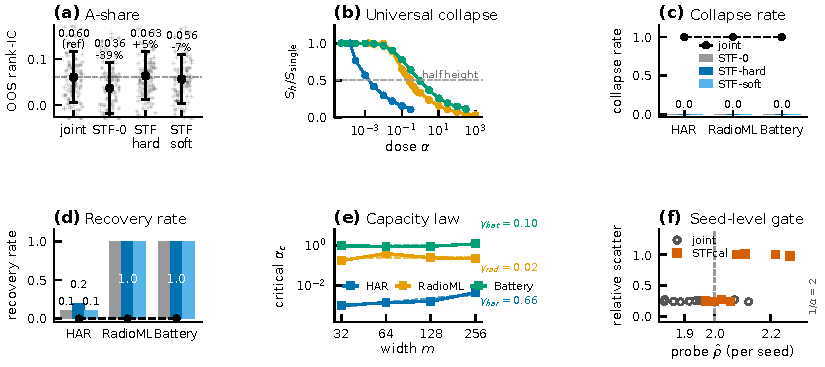
\includegraphics[width=\columnwidth]{figures/unified_all.pdf}
\caption{Diagnostics and interventions across domains. Shading marks the operational scatter criterion $0.3$. (a) Dose--scatter curves at $m=128$; the dotted line marks the half-height crossing, distinct from the collapse criterion $0.3$. (b) Width-dependent half-height crossings and log--log OLS fits (nine widths for HAR and battery, four for RadioML). (c) NYUv2 at $\alpha=0.5$: paired outcomes share the same warm-up probe coordinate; the dotted line marks $1/\alpha=2$. (d,e) Collapse and task-recovery rates from Table~\ref{tab:unified_repair}. (f) Financial rank-IC: each point averages ten seeds within one temporal fold; thin lines pair folds, and large markers show the mean with population s.d. across ten folds.}
\label{fig:unified}
\end{figure}

\section{Experiments}\label{sec:experiments}

\subsection{Unified Protocol}\label{sec:unified_protocol}

Controlled comparisons use the same gradient diagnostic and relative-scatter criterion (Algorithm~\ref{alg:stf}), with architecture and batch details specified per experiment. The default encoder is a three-layer MLP of width $m$. Primary tasks use accuracy or RMSE; the auxiliary \emph{variance-shrinkage toxifier}, $L_{tox}=\mathrm{Var}_b[W_k h]$, uses $K=3$ seeded random projections and realizes Definition~\ref{def:degmin}. Default training uses Adam ($\mathrm{lr}=10^{-3}$, batch $256$), bf16 autocast on an NVIDIA A100 80\,GB, and $5$--$10$ seeds per configuration. We define operational collapse by $\mathcal{S}_h<0.3\,\mathcal{S}_{single}$, where
\begin{equation}
\mathcal{S}_h=\mathbb E_b\!\left[\mathrm{std}_j\!\left(h_j^{(b)}-\mathbb E_{b'}[h_j^{(b')}]\right)\right],
\label{eq:cross_sample_scatter}
\end{equation}
is anchored to the same-seed single-task reference. The implementation averages standard deviations across features after centering examples (sample correction $m-1$). This coordinate-dependent proxy differs from covariance trace and from averaging per-feature standard deviations across examples. It can miss variation along the all-ones feature direction; operational collapse therefore does not establish total variance collapse. We report collapse rate, recovery rate, the diagnostic $\rho$, and relative scatter $\mathcal{S}_h/\mathcal{S}_{single}$; Table~\ref{tab:domains} lists the domains. The toxifier's combined rank and normalization require separate width audits; Section~\ref{sec:bmtl} tests real auxiliary heads. Across ten seeds per domain, \textsc{stfcal} increases scatter over joint training at $p<0.01$ (Wilcoxon; $|d_z|>20$). Battery SOH RMSE improves by $0.050$ (95\% CI $[0.033,0.067]$, $d_z=1.8$). All four scatter tests and the battery SOH test survive Holm correction within this five-test family (\texttt{paired\_stats.py}). Unless identified as a confidence interval, $\pm$ denotes population standard deviation across the stated seeds or cells. Financial fold-seed cells share data and are not independent replicates.

\subsection{Cross-Domain Validation}\label{sec:validation}

We study A-share ranking (Appendix~\ref{app:finance})\label{sec:finance}, UCI-HAR\label{sec:har}, RadioML2016.10A\label{sec:radioml}, battery health on the NASA PCoE and MATR archives~\citep{nasa_battery,severson2019data}\label{sec:battery}, and NYUv2 dense perception\label{sec:nyu} (Appendix~\ref{app:nyu}), with CelebA as an additional check. The financial application uses real auxiliary heads and a separate walk-forward protocol. In the high-dose controlled comparisons, filtering reduces operational collapse from $1.0$ to $0.0$; this does not extend to every method or boundary dose. Where shrinkage also harms the primary task, RadioML accuracy recovers from $0.091$ to approximately $0.33$, and battery log-SOH RMSE improves from $0.611$ to $0.305$ (Figure~\ref{fig:battery_repair}; Table~\ref{tab:unified_repair}).

Task metrics reveal shrinkage unevenly. HAR still attains approximately $0.95$ accuracy at relative scatter $0.05$. In one MATR protocol, an encoder with relative scatter $0.0052$ achieves lower SOH RMSE than detachment ($0.82$ versus $1.51$). A trainable head can compensate for reduced representation amplitude, so small scatter need not imply constant predictions. We therefore examine task error, prediction variance, and representation covariance together.

\subsection{Battery Health and Remaining-Life Prediction}\label{sec:bmtl}

Battery prediction provides an application with a temporal encoder, two target tasks, and practical auxiliary heads. The model predicts SOH and RUL jointly, allowing us to test whether controlling auxiliary updates improves either task.

A \textsc{TSMixer} block~\citep{ekambaram2023tsmixer} and a gated state-space block~\citep{gu2022s4,gu2023mamba} map each cell's per-cycle window to $h\in\mathbb{R}^{d}$. The representation feeds SOH ($L_2$) and RUL ($L_1$) heads, plus reconstruction and distributional auxiliaries evaluated empirically (Appendix~\ref{app:moved}).

RUL supervision uses absolute error for observed lifetimes and a one-sided hinge for censored lower bounds. The historical evaluation, however, reports MAE over both types of target and selects checkpoints using evaluation SOH, including for the RUL-only reference. Its RUL scores therefore do not estimate uncensored lifetime error. The corrected protocol selects checkpoints on validation data and reports observed-only MAE and censored shortfall separately.

Under the corrected MATR protocol, detachment improves both tasks (Table~\ref{tab:bmtl_corrected}). Relative to joint training, paired mean differences are $-3.47$ SOH percentage points (95\% $t$ interval $[-4.20,-2.74]$) and $-34.8$ observed-RUL cycles ($[-57.8,-11.8]$), closing $70\%$ of the SOH gap to the SOH-only reference. These intervals capture ten initializations on one cell split, not uncertainty over new cell populations. Because several protocol choices changed together, the revised ordering cannot be attributed to censoring alone. Selective filtering does not outperform detachment; the rank arm's large covariance trace and low effective rank do not establish spectral saturation. On NASA, detachment improves SOH, but the observed-RUL difference is inconclusive (Appendix~\ref{app:tables}).

\begin{table}[t]
\centering
\caption{Corrected MATR test results: ten initialization seeds on a fixed cell-disjoint split, with validation-based checkpoint selection. $S=\operatorname{tr}\operatorname{Cov}(H)$; relative $S$ is the mean same-seed ratio to the SOH-only reference; PR is participation rank. Censored shortfall measures lower-bound violations in cycles. Table~\ref{tab:battery_evidence} reports uncertainty.}
\label{tab:bmtl_corrected}
\small
\resizebox{\columnwidth}{!}{\begin{tabular}{lrrrrrr}
\toprule
Mode & SOH RMSE\% $\downarrow$ & obs.\ RUL MAE $\downarrow$ & shortfall $\downarrow$ & $S$ & relative $S$ & PR \\
\midrule
SOH-only & $0.61$ & --- & --- & $1.01$ & $1.00$ & $1.35$ \\
\textsc{joint} & $5.57$ & $81.5$ & $17.60$ & $2.86$ & $3.55$ & $2.49$ \\
\textsc{stf-0} & $\mathbf{2.10}$ & $\mathbf{46.7}$ & $\mathbf{2.06}$ & $4.77$ & $6.24$ & $1.86$ \\
\textsc{stfcal} & $2.71$ & $63.6$ & $5.73$ & $1.40$ & $1.89$ & $2.03$ \\
\textsc{stfcalrank} & $4.98$ & $107.6$ & $17.57$ & $617.90$ & $651.77$ & $1.21$ \\
\bottomrule
\end{tabular}}
\end{table}

A separate HAR reconstruction experiment tests basis selection at $\alpha=12$. Both bases open the gate in the same four of ten seeds. Among those seeds, the auxiliary-gradient basis removes $30.75$ directions on average, compared with PCA's $62.0$, at similar accuracy across all ten seeds (Table~\ref{tab:realbasis}). This supports basis sensitivity without establishing superiority over joint training or globally minimal deletion. Historical battery and regime-weighting results appear in Appendix~\ref{app:moved}.

% Generated by repro/scripts/real_basis_evidence_audit.py
\begin{table}[t]\centering\small
\caption{Real HAR reconstruction ($m=R=64$, ten seeds). Candidate rank includes closed-gate seeds; active rank averages only gate-open seeds. Accuracy and scatter average all ten seeds. The two bases open on the same seeds. No superiority over joint training or global rank optimality is inferred.}
\label{tab:realbasis}
\resizebox{\columnwidth}{!}{\begin{tabular}{clrrrrr}\toprule
$\alpha$ & basis & gate open & candidate rank & active rank & rel.\ scatter & accuracy \\
\midrule
$12$ & pca & $4/10$ & $57.0$ & $62.00$ & $0.842$ & $0.9492$ \\
$12$ & aux & $4/10$ & $22.6$ & $30.75$ & $0.811$ & $0.9497$ \\
$30$ & pca & $8/10$ & $62.8$ & $63.62$ & $0.754$ & $0.9512$ \\
$30$ & aux & $8/10$ & $44.1$ & $47.88$ & $0.746$ & $0.9531$ \\
$100$ & pca & $10/10$ & $64.0$ & $64.00$ & $0.630$ & $0.9524$ \\
$100$ & aux & $10/10$ & $59.4$ & $59.40$ & $0.654$ & $0.9520$ \\
\bottomrule\end{tabular}}\end{table}


\subsection{Battery Ablations}\label{sec:bmtl_ablation}

Appendix~\ref{app:tables} reports historical ablations of censoring-aware supervision (Table~\ref{tab:cens_ablation}), auxiliary weight, and regime weighting. At $d=128$, increasing the auxiliary dose worsens joint SOH RMSE from $1.36$ to $6.58$\%, whereas the detached results are unchanged. A ten-seed NASA experiment additionally evaluates the three-factor regime weighting.





\subsection{Comparison with Conflict-Resolution Methods}\label{sec:conflict_ablations}

The four real-head comparisons show that gradient conflict and contraction need not coincide. Across ten seeds, $|\cos(g_p,g_a)|\le0.06$ with both dot-product signs represented. Yet for the collapsing SNR head, $88\%$ of $\|g_a\|$ projects onto $u_c$, compared with $1$--$14\%$ for the other heads. We also compare ten multi-task optimizers at matched doses and seeds, using their published defaults: PCGrad, CAGrad, FAMO, MGDA, Aligned-MTL, IMTL-G, Nash-MTL, uncertainty weighting, GradNorm, and IMTL-L. All retain a collapse rate of $1.0$ in the three controlled domains (Table~\ref{tab:conflict}). On HAR, seven yield lower accuracy than plain summation ($0.945$), including four at $0.18$--$0.42$. Separate battery-head results appear in Table~\ref{tab:conflict_num}. In the financial comparison, six-fold mean rank-IC ranges from $-0.022$ to $+0.032$ across methods, versus $-0.004$ for summation, within the observed fold variation.


Applying a filter before a conflict operator preserves scatter at the tested high doses (Table~\ref{tab:compose}). These experiments establish compatibility in this order; the reverse order was not tested (Appendix~\ref{app:moved}).


% ═══════════════════════════════════════════════════════════════════
% 7. ANALYSIS
% ═══════════════════════════════════════════════════════════════════
\section{Analysis and Discussion}\label{sec:analysis}

We examine width scaling, the interpretation of the diagnostic, and transfer to real auxiliary heads.

\subsection{Width Scaling}\label{sec:capacity_law}

We fit $\log\alpha_c=\gamma\log m+c$ to empirical half-height crossings. Four-width slopes are $2.43$ for the fixed-per-head-rank schedule, $0.66$ for HAR, $0.10$ for battery, and $0.02$ for RadioML; nine-width fits give $0.38$ for HAR and $-0.06$ for battery. These describe crossing locations, not independently identified restoration or toxic-rank exponents. Inferring $\beta$ from them would assume the law being tested. A joint fit to the synthetic family gives $\gamma_0=2.50$ (nominal 95\% CI $[1.94,3.06]$); shared seeds and identical pivot curves limit this cell-level inference. An unconstrained fit does not reject $\gamma=\gamma_0(1-\beta)$, with implied dilution factor $0.78$--$1.03$ versus $1.00$. However, fixed per-head ranks $r=4,8,16$ give slopes $-0.31$, $+0.45$, and $+3.02$, and changing the width set moves $\gamma_0$ over $[1.35,2.87]$. Exact-rank controls also reveal normalization dependence (Appendix~\ref{app:proofs}). The data therefore support a conditional scaling trend, not a universal exponent or an independently established rank-dilution law.

\subsection{Diagnostics and Their Limits}\label{sec:diagnosis}

Task error can remain stable despite substantial scatter loss. The projected-norm ratio measures magnitude, whereas the parameter-space identity measures signed contraction. Probe--crossing agreement at one width does not imply a shared width exponent, and prediction normalization provides no general recovery guarantee.

\subsection{Calibration Across Real Heads}\label{sec:real_aux}\label{sec:negatives}

Table~\ref{tab:real_aux} shows heterogeneous outcomes. Neither reconstruction head crosses the collapse threshold at the tested dose, whereas high-dose SNR regression does. Only full detachment avoids operational collapse in all ten SNR seeds; the selective implementations do not recover its accuracy consistently. At RadioML dose $1$, the calibrated gate can remain closed despite joint collapse. Basis drift and limited probe depth are possible explanations, not established causes. In the historical MATR experiment, increasing the rank cap from $3$ to $32$ leaves SOH RMSE near joint training ($5.26$ versus $5.24$), while the radial arm reaches $1.77$. Because $32$ remains below the feature width, this result shows that the tested increase is insufficient, without ruling out a larger cap.

These findings define the diagnostic's scope: width slopes depend on the experimental family, norm ratios do not encode the sign of variance change, and calibration depends on both basis and measurement time. Each requires validation for the intended operating regime.

\begin{table}[t]
\centering
\caption{Real auxiliary heads ($m=64$, ten seeds): mean primary accuracy with collapse rate in parentheses. The calibrated gate remains closed for both reconstruction heads. With SNR regression, all joint seeds collapse; selective variants do not restore accuracy, and only full detachment avoids the collapse criterion in every seed.}
\label{tab:real_aux}
\small
\resizebox{\columnwidth}{!}{%
\begin{tabular}{lcccccc}
\toprule
Auxiliary head & $\alpha$ & \textsc{joint} & \textsc{stf-0} & \textsc{stf-hard} & \textsc{stf-soft} & \textsc{stfcal} \\
\midrule
HAR input-reconstruction & $0.1$ & $.942$ ($0.0$) & $.943$ ($0.0$) & $.942$ ($0.0$) & $.942$ ($0.0$) & $.942$ ($0.0$) \\
HAR subject-ID probe & $0.1$ & $.941$ ($0.0$) & $.943$ ($0.0$) & $.944$ ($0.0$) & $.943$ ($0.0$) & $.942$ ($0.0$) \\
RadioML I/Q-reconstruction & $3000$ & $.343$ ($0.0$) & $.307$ ($0.0$) & $.329$ ($0.0$) & $.327$ ($0.0$) & $.315$ ($0.0$) \\
RadioML SNR regression & $3000$ & $.205$ ($1.0$) & $\mathbf{.307}$ ($\mathbf{0.0}$) & $.208$ ($1.0$) & $.200$ ($0.9$) & $.199$ ($0.1$) \\
\bottomrule
\end{tabular}}
\end{table}


% ═══════════════════════════════════════════════════════════════════
% 8. CONCLUSION
% ═══════════════════════════════════════════════════════════════════
\section{Conclusion}\label{sec:conclusion}

Gradient toxicity exposes a failure that pairwise conflict criteria do not directly measure: auxiliary updates can contract a shared representation even without gradient opposition. An exact parameter-space identity diagnoses instantaneous contraction, while conditional scalar and spectral models distinguish it from eventual collapse. A frozen warm-up probe identifies useful intervention regimes, but its transfer depends on basis, timing, and dose. Under corrected MATR evaluation, detachment improves SOH and observed RUL; on HAR reconstruction, an auxiliary-gradient basis substantially reduces deletion rank at similar accuracy. These results support monitoring representation variation alongside task metrics and comparing selective deletion with detachment and scalar attenuation. The guarantees remain confined to their stated assumptions; the empirical contribution is a diagnostic and a tested family of interventions.




\clearpage
\section*{AI Use Statement}
Generative AI tools assisted with drafting, language editing, code, literature retrieval, proof development, and figure design. Executable counterexamples exposed overly broad theoretical claims, which were revised to state their assumptions. Figures were redrawn from recorded experimental results. The authors remain responsible for verifying the final text, claims, code, and artifacts.

\section*{Ethics Statement}
We use existing datasets: UCI-HAR, RadioML2016.10A, the NASA PCoE and MATR battery archives, public A-share market data, NYUv2, and CelebA. We collected no new human-subject data. The HAR identity auxiliary is evaluated as a training-head probe, not a held-out privacy attack. Battery prediction is safety-relevant; Section~\ref{sec:negatives} describes the observed limitations, and deployment requires task-specific validation.






\section*{Reproducibility Statement}
Appendices~\ref{app:proofs}--\ref{app:general} give the assumptions and scope of the theoretical results. The repository provides experiment code, per-seed records, counterexample checks, generator audits, and the corrected battery validation protocol. Historical battery results selected checkpoints on the evaluation split and are exploratory, rather than independent test estimates. Code and records are available in the anonymized repository: \url{https://github.com/code-2026l/RepFix}.

\bibliographystyle{iclr2027_conference}
\bibliography{RepFix_ICLR2027}


% ═══════════════════════════════════════════════════════════════════
% APPENDICES
% ═══════════════════════════════════════════════════════════════════
\clearpage
\appendix
The appendices cover the financial application (Appendix~\ref{app:finance}), proofs and scaling analyses (Appendix~\ref{app:proofs}), generalizations and finite-sample theory (Appendix~\ref{app:general}), additional tables and protocols (Appendix~\ref{app:tables}), NYUv2 (Appendix~\ref{app:nyu}), supplementary experiments (Appendix~\ref{app:moved}), and matched-dose regularization baselines (Appendix~\ref{app:reg}).
\section{Financial Ranking Application}\label{app:finance}

The failure was first observed in multi-task equity selection. A production model combined a pairwise-ranking head with distributional (MDN~\citep{bishop1994mixture}), reconstruction (AE), and view-contrastive (SCARF-style~\citep{bahri2022scarf}) auxiliaries over a shared encoder of A-share factors. After deployment, with the training objective unchanged, predicted rankings became nearly constant. Cross-sectional prediction spreads fell by approximately $93\%$ relative to validation, although individual training losses remained low. This observation motivates measuring representation and prediction variation alongside loss; it does not by itself identify a constant attractor or vanishing gradients.

The financial application uses a separate walk-forward model with real distributional, reconstruction, and contrastive heads. The released R5fin records set \texttt{fixed\_aux=0}; Table~\ref{tab:finance_repair} therefore does not replicate the controlled variance toxifier. Across ten folds and ten initialization seeds, mean out-of-sample (OOS) rank-IC is $0.060$ for joint training, $0.036$ for detachment, $0.063$ for the hard gate, and $0.056$ for the soft gate. After averaging seeds within each fold, paired differences from joint are $-0.0237$, $+0.0029$, and $-0.0042$, respectively. Two-sided Wilcoxon $p$ values are $0.037$, $0.432$, and $0.695$; none survives Holm correction over the three comparisons. Because temporal folds may remain dependent, these tests are sensitivity analyses rather than independent-population inference. The results suggest a possible cost of indiscriminate detachment without establishing retention of a particular useful subspace. The script \texttt{finance\_fold\_audit.py} reproduces the comparisons from all 40 source files.

In the separate synthetic testbed, initialization probes give $\rho=0.74\pm0.19$ over 12 seeds and predicted critical weight $\alpha_c=\langle1/\rho\rangle=1.45\pm0.37$, consistent with the observed onset. Other domains use the projected-gradient diagnostic of Definition~\ref{def:toxicity}, but its numerical value depends on the task, encoder, and calibration time.

\section{Proofs and Additional Analysis}\label{app:proofs}

\subsection{Statements Deferred from the Main Text}
We formalize several statements discussed in the main text. Theorem numbering continues from the main text.


\begin{proposition}[Sufficient conditions for gradient vanishing]\label{prop:gradient_vanishing}
For a differentiable prediction map with Jacobian $J$ and output loss gradient $\ell$, the parameter gradient vanishes iff $J^\top\ell=0$. Sufficient conditions are $\ell=0$, or identical Jacobian rows together with $\mathbf1^\top\ell=0$. Equal prediction values alone imply neither condition.
\end{proposition}
\begin{proof}
Apply the chain rule. For a counterexample to the stronger assertion, $\hat y_i=\theta x_i$ is constant at $\theta=0$ but has Jacobian rows $x_i$. The pairwise logistic loss $\log(1+e^{-(\hat y_1-\hat y_2)})$ has output gradient $(-1/2,1/2)$ at a tie, so its parameter gradient is $(x_2-x_1)/2$, generally nonzero.
\end{proof}

\begin{proposition}[Scope of positive attenuation]\label{prop:minimality}
Under Theorem~\ref{thm:transition}, a fixed positive multiplier $q$ leaves a finite threshold $\alpha_c/q$ but can prevent the transition at a specified dose. A dose-dependent positive multiplier can keep the effective dose subcritical for every $\alpha$: for $0<\epsilon<1$, take $q(\alpha)=(1-\epsilon)/(1+\alpha/\alpha_c)$.
\end{proposition}
\begin{proof}
Substitute $q\alpha$ for $\alpha$. The proposed choice gives $q\alpha/\alpha_c=(1-\epsilon)\alpha/(\alpha+\alpha_c)<1$. A positive stable equilibrium remains, although its lower basin boundary persists. Preserving gradient direction therefore does not imply that positive task weighting must fail.
\end{proof}

\begin{proposition}[Rank-dilution scaling]\label{prop:rank_dilution}
Assume the effective ratio scales as $\rho_\star\asymp(m_\Pi/m)^{\gamma_0}$, $\gamma_0\ge1$, and $m_\Pi\propto m^\beta$, $0\le\beta<1$. Then $\alpha_c=1/\rho_\star$ implies
\begin{equation}
\gamma \;=\; \gamma_0\,(1-\beta), \qquad \gamma_0 \ge 1,
\label{eq:rank_dilution}
\end{equation}
The separable scaling is assumed; rank alone does not imply it. More generally, restoration $\asymp m^a$ and contraction $\asymp m^b m_\Pi^c$ yield $\gamma=a-b-c\beta$, with the displayed form requiring $c=a-b=\gamma_0$. If the toxic norm scales as $m_\Pi^p$, then $c=2p$ only when contraction depends quadratically on that norm and has no additional rank dependence. The equality $\gamma_0=2p$ further requires $a-b=2p$. Neither exponent is identified by the toxic eigenvalue spectrum alone. A fixed effective rank gives $\beta=0$; a fixed per-head output dimension need not.
\end{proposition}

\begin{corollary}[Composition of rank-one PSD operators]\label{cor:additive}
Let $T=\sum_k\rho_k u_ku_k^\top$, with unit $u_k$ and $\rho_k\ge0$, in common restoration-normalized coordinates. If the directions are mutually orthogonal, $\lambda_{\max}(T)=\max_k\rho_k$; if aligned, it is $\sum_k\rho_k$. An additional orthogonal direction leaves the maximum unchanged only if its coefficient does not exceed the previous maximum.
\end{corollary}
\begin{proof}
For orthogonal directions, the $u_k$ are eigenvectors. For aligned directions, the sum is a single rank-one operator. Neither case establishes the geometry of the production model's heads.
\end{proof}

For an explicit scalar example, take $b(\sigma)=\lambda\sigma^2/(1+\sigma^2)$. Then
\begin{equation}
\sigma_\pm=\frac{\lambda\pm\sqrt{\lambda^2-4(\alpha\kappa)^2}}{2\alpha\kappa},\qquad \alpha_c=\lambda/(2\kappa).
\label{eq:fp}
\end{equation}
This verifies the fold and its basin dependence. Radial auxiliary behavior,
\begin{equation}
g_a=\kappa\delta h+o(\|\delta h\|),
\label{eq:radial}
\end{equation}
requires isotropic curvature; stationarity at a constant representation is insufficient. For a general encoder, the Jacobian still determines its effect on variance through \eqref{eq:signed_variance}. In discrete time, linearizing a scalar stable equilibrium~\citep{strogatz1994nonlinear} with derivative $-\ell$ gives
\begin{equation}
e_{t+1}=(1-\eta\ell)e_t,\qquad 0<\eta\ell<2,
\label{eq:parallel_contraction}
\end{equation}
where $e_t$ is a deviation from that equilibrium, not total representation scatter.

Power-law spectra do not determine the capacity exponent. For eigenvalues $\lambda_i=C i^{-(1+s)}$ with $C$ independent of rank,
$\|A_r\|_F^2=C^2\sum_{i=1}^r i^{-2(1+s)}$. Hence the Frobenius norm is bounded for $s>-1/2$, grows as $\sqrt{\log r}$ for $s=-1/2$, and as $r^{-s-1/2}$ for $s<-1/2$. A decaying spectrum ($s>-1$) therefore has power exponent at most $1/2$; for the commonly intended $s>0$ it has exponent zero. The trace instead involves $\sum_i i^{-(1+s)}$, and the operator norm is $C$ for a decreasing spectrum. Rank-dependent normalization $C(r,m)$ changes these conclusions. Thus neither a universal $\gamma_0(s)$ nor $\gamma_0=2p$ follows without specifying the norm, normalization, restoration and coupling to dynamics. Concretely, if $\kappa\asymp m^b\|A_r\|^q$, $\|A_r\|\asymp r^p$, and $r\asymp m^\beta$, then $\gamma=a-b-qp\beta$. The restricted form $\gamma_0(1-\beta)$ requires $a-b=qp=\gamma_0$. Hence $\gamma_0=2p$ holds only under the additional quadratic coupling $q=2$ and matching restoration exponent $a-b=2p$; these are not implied by the measured width slope.

The original two-head generator has $W_k\in\mathbb R^{m\times r}$ with independent entries of variance $1/r$. Its combined span has rank $\min(m,2r)$ almost surely. For the averaged quadratic loss the sample-normalized Hessian is $A=2\sum_k W_kW_k^\top/(2r)$, with $\mathbb E A=2I/r$. At $r=32$, widths $32,64,128,256$ therefore have ranks $32,64,64,64$. Fixed per-head rank is not fixed combined rank over this range, and changing $r$ also changes curvature. The supplied orthonormal control instead constructs $A=Q\operatorname{diag}(\lambda)Q^\top$ at exactly specified rank and normalization.

The RS1 experiment fixes per-head ranks $r\in\{4,8,16\}$ across widths $32,48,64,96$, giving combined ranks $8,16,32$. With anchor $3\times10^{-4}$, descriptive half-height slopes are $-0.31$, $0.45$, and $3.02$. Minimum relative scatter ranges are $0.040$--$0.068$, $0.013$--$0.018$, and $0.0056$--$0.0132$, respectively: some curves contract without reaching a near-zero floor. Using the unpenalized anchor changes the slopes to $0.65$, $5.55$, and $3.88$. This rank and anchor sensitivity does not support a single universal exponent. The released analyzer retains all twelve curves and reports crossings separately from scatter floors.

The orthonormal control constructs the sample-normalized auxiliary Hessian $A=Q\operatorname{diag}(\lambda)Q^\top$ at exact rank $r$ and verifies its amplitude. Three normalizations hold different quantities fixed: $\lambda=1$ fixes curvature per direction, so the Frobenius norm grows as $\sqrt r$; $\lambda=1/r$ fixes the trace; and $\lambda=1/\sqrt r$ fixes the Frobenius norm. The training grid tests the first two at $m\in\{32,64,128\}$, $r\in\{4,16\}$, seven doses, and three seeds, holding the loss, optimizer, and data generator otherwise fixed. Three observations follow. First, at fixed width and per-direction curvature, the $r=16$ crossing is lower than the $r=4$ crossing by factors of $4.8$ at $m=64$ and $228$ at $m=32$. Second, the fitted width slope for $r=4$ changes from $-0.29$ under $\lambda=1$ to $+0.91$ under $\lambda=1/r$. Third, minimum scatter is $3.5$--$11\%$ of the healthy reference for $r=4$, versus $0.4$--$1.1\%$ for $r=16$. Thus normalization affects the estimated exponent even when rank is controlled exactly. Each three-width fit has only one residual degree of freedom and cannot identify a precise exponent. The commands \texttt{controlled\_rank\_scan.py --self-test} and \texttt{run\_controlled\_rank\_grid.py} verify the construction and reproduce the twelve configurations. The historical squared pairwise hinge has zero margin, so tied scores can attain zero primary loss. These controls concern that objective; they do not establish the same transition for informative ranking objectives. The separate \texttt{--primary-loss logistic} option removes this degeneracy, but no unfinished logistic sweep is counted as evidence.


The synthetic testbed uses random toxic projections of rank $\lfloor m/2\rfloor$ and a low-rank primary task with $2$--$8$ active directions across seeds (mean $5.3$). It sweeps 17 logarithmically spaced doses over $[3\times10^{-4},10]$ at six widths $m\in\{8,\dots,256\}$ under a pairwise-ranking loss. The toxic-rank schedule is proportional to width. The relative half-height rule gives $\gamma=0.07$ across six widths and $\gamma=0.01$ across the four widths used below. This nearly flat trend is consistent with the restricted law at $\beta=1$, but does not independently establish that law.

Using a fixed absolute scatter threshold instead gives $\gamma=1.53$ ($R^2=0.91$) on the same curves. At $\sigma_h=1.5\times10^{-3}$, the crossing depends on the width-dependent healthy amplitude: the fixed-rank family has $\sigma_h(0)\propto m^{0.95}$. The absolute rule also gives nearly constant slopes $1.94,2.02,2.04,1.96,1.89$ across rank schedules $\beta=0,\dots,1$, varying by only $0.15$ and largely masking schedule dependence. Using relative crossings, the fixed-per-head-rank family instead gives $\gamma_0=2.43$ ($R^2=0.90$, four widths). Its combined span can still grow as $\min(m,2r)$, so this is not an exact fixed-effective-rank estimate.

Both synthetic families extend the dose grid to $\alpha=0$ (21 points), using four widths $m\in\{32,64,128,256\}$, five seeds, and 800 epochs. The fixed-rank family is the $\beta=0$ case with constant per-head rank $r$. A corresponding ten-seed run yields crossings differing by $+3.1\%,+1.8\%,-5.8\%,+19.7\%$ across these widths. This comparison quantifies sensitivity to seed count, including variation in the healthy anchor at larger widths.

Two checks qualify the crossing estimator. First, a half-height crossing can occur without near-total collapse. For fixed per-head rank $r\le4$, scatter plateaus at $2$--$23\%$ of its healthy value; only $r\ge8$ reaches a floor of at most $0.9\%$. These floors must be distinguished from the operational $0.3$ collapse threshold. Second, the synthetic fits use the first penalized dose, $\alpha=3\times10^{-4}$, as the anchor. The unpenalized value is set by the ranking loss, is shared across toxic ranks, and lies $30$--$40\%$ above the penalized trend. Varying the anchor over $\alpha\in[0,3\times10^{-3}]$ preserves the decreasing ordering of $\gamma(\beta)$: $\gamma_0\in[1.55,3.23]$ at $\beta=0$, versus $\gamma(1)\in[-0.06,+0.74]$. The ordering is more stable than the fitted coefficients.

The rank-schedule fits below test a restricted scaling hypothesis. Substituting $m_\Pi\asymp m^\beta$ into an independently established $\alpha_c\asymp(m/m_\Pi)^{\gamma_0}$ gives $\gamma=\gamma_0(1-\beta)$; it does not establish the premise. Back-solving $\beta$ from measured $\gamma$ cannot serve as an independent measurement of toxic rank. The original generator audit further limits interpreting its per-head rank schedule as an effective-rank schedule.

Crossing rules affect the fitted magnitudes. For HAR, an absolute threshold $T\in[0.20,0.50]$ gives $\gamma\in[0.66,0.82]$, compared with $0.66$ under the four-width relative rule. Battery requires a grid that reaches a healthy branch: earlier sweeps started at $\alpha=300$, where relative scatter was already $0.07$--$0.11$, making thresholds left-censored. Extending to $\alpha\in[10^{-4},300]$ with five seeds gives a healthy branch at $\alpha\le10^{-3}$ (relative scatter $1.000\pm0.005$) and crossings $0.95,0.89,0.90,1.18$ at $m=32,\dots,256$. The fitted slope is $\gamma_{\mathrm{bat}}=0.10$ ($R^2=0.43$), varying over $[-0.10,+0.12]$ across crossing rules. These four widths are consistent with weak width dependence but do not resolve a precise exponent.

Treating each width's crossing as one observation gives four-width OLS 95\% intervals $[-0.07,+4.93]$ for the $\beta=0$ schedule, $[-0.16,+1.49]$ for HAR, $[-0.24,+0.43]$ for battery, and $[-1.16,+1.20]$ for RadioML. None excludes zero. Interior schedules yield positive slopes: $2.57$ (CI $[0.87,4.27]$) at $\beta=0.25$ and $1.86$ ($[0.81,2.91]$) at $\beta=0.50$; $\beta=1$ remains consistent with zero. At the reported anchor, all four remaining schedule intervals contain $\gamma_0(1-\beta)$, whereas the $\beta=0.75$ interval excludes it at anchor $10^{-4}$. These results support schedule dependence without identifying an anchor-independent coefficient.

The denser SYN8 family supplies $26$ completed $(m,\beta)$ cells, ten seeds each. Since $r(64)=32$ for every schedule, we fit $\log\alpha_c=c+\gamma_0(1-\beta)\log(m/64)$. At anchor $3\times10^{-4}$, the constrained fit gives $\gamma_0=2.50$ (nominal OLS $95\%$ CI $[1.94,3.06]$). Across anchors $\{10^{-4},3\times10^{-4}\}$ and inclusion/exclusion of $m=128$, all four conditional intervals exclude zero (lowest bound $1.04$). In the unconstrained model $c+a x+b\beta x$, $x=\log(m/64)$, every interval for $a+b$ contains zero and $-b/a=0.78$--$1.03$: the linear form is not rejected, not established. These are cell-level fit intervals, not independent-seed uncertainty: the schedules share seeds and the $m=64$ curves are identical. Joint/anchor-row point estimates range from $1.35$ to $2.87$. At $m\ge96$ the sampled curve never resolves the collapsed floor; half-height crossings interpolate the observed decline, not a verified collapse threshold. Thus SYN8 sharpens a conditional trend without supplying a precise physical exponent. \texttt{synth\_beta\_joint.py} reproduces the fits.

Nine-width HAR and battery sweeps use $m\in\{16,24,32,48,64,96,128,192,256\}$ with the same driver, seeds, epochs, and dose grids. Shared configurations agree to floating-point precision (maximum difference $2\times10^{-16}$). HAR gives $\gamma_{\mathrm{HAR}}=0.38$ (95\% CI $[+0.10,+0.67]$, $R^2=0.60$, $n=9$); excluding the two narrowest widths gives $0.60$. Battery gives $\gamma_{\mathrm{bat}}=-0.06$ (CI $[-0.17,+0.06]$), consistent with weak width dependence. The denser grid narrows conditional fit intervals but does not eliminate crossing uncertainty. For example, HAR at $m=32$, $\alpha=10^{-3}$ has relative scatter $0.5026\pm0.0524$, placing the half-height crossing close to a sampled grid point and making interpolation sensitive to seed variation. We report both four- and nine-width estimates rather than treating either as an identified dynamical exponent.

We also examine probe scaling across encoders. Repeating calibration with a Transformer at $m\in\{32,64,128\}$ and ten seeds gives probe exponents $-0.93$ for HAR ($R^2=0.99$), $+0.39$ for battery ($R^2=0.87$), and $-0.17$ for RadioML ($R^2=0.79$). The corresponding MLP values are $-1.63$ ($R^2=0.96$), $+0.67$ ($R^2=0.86$), and $+0.28$ ($R^2=0.40$). Signs agree for HAR and battery; RadioML is consistent with zero for both encoders, and the 95\% intervals overlap in all three domains. This is evidence of broadly similar probe trends in the tested encoders, not architecture invariance. The script \texttt{probe\_exponent.py} reproduces the analysis.

Probe exponents and scatter-crossing exponents estimate different quantities. Their MLP point estimates agree in sign for RadioML ($+0.28$ versus $+0.02$), but disagree for HAR ($-1.63$ versus $+0.38$) and battery ($+0.67$ versus $-0.06$). A half-height crossing locates a dose at which trained scatter reaches half its reference value; the probe estimates $1/\hat\rho$ at the warm-up anchor. Agreement within a factor of a few at one width (a factor of $7$ for NYUv2 at $m=64$) does not imply agreement in width scaling. Negative probe slopes do not satisfy the restricted nonnegative exponent assumed in \eqref{eq:rank_dilution}, but that assumption is not a general constraint on empirical slopes. Section~\ref{sec:capacity_law} therefore reports crossing exponents, while Appendix~\ref{app:nyu} reports probe values as calibration statistics.

Several sweeps show bimodal per-seed scatter near an empirical crossing. This is consistent with multiple outcomes but does not uniquely identify a saddle-node bifurcation; initialization, finite training time and optimization can also generate heterogeneous outcomes.

The original GPU experiments use fixed integer seeds, bf16 autocast with TF32 matrix multiplication, and Adam ($\mathrm{lr}=10^{-3}$, batch 256) on an NVIDIA A100 80\,GB. Exceptions are specified with their protocols. Operational collapse means scatter below $0.3$ times the same-seed single-task reference; the released recovery rate compares each seed with the mean joint-training metric. Code, seeds, hyperparameters, and per-fold results are included in the repository.

\section{Generalizations and Finite-Size Theory}\label{app:general}

\begin{proposition}[Fixed attenuation in a specified model]\label{prop:attenuation}
For $T\succeq0$ in restoration-normalized coordinates, uniform attenuation $T\mapsto(1-\lambda)T$, $0\le\lambda<1$, multiplies the first-modal-contraction threshold by $1/(1-\lambda)$. At fixed dose the smallest $\lambda$ meeting $\alpha(1-\lambda)\|T\|\le1$ is $\max(0,1-1/(\alpha\|T\|))$ when $\alpha\|T\|>0$.
\end{proposition}
\begin{proof}
All eigenvalues scale by $1-\lambda$; solve the displayed inequality. This statement concerns a fixed PSD model, not arbitrary signed or nonsymmetric filtered dynamics.
\end{proof}

\begin{theorem}[Annihilation by orthogonal compression]\label{thm:filters}
Let $T\succeq0$, $U=\mathrm{range}(T)$, and $Q=I-P_S$ be an orthogonal projector. Then $QTQ=0$ iff $U\subseteq S$. Among such deletions the unique smallest deleted subspace is $U$, and $I-P_U$ preserves its orthogonal complement. This is an algebraic statement about two-sided compression.
\end{theorem}
\begin{proof}
$QTQ=(T^{1/2}Q)^\top(T^{1/2}Q)=0$ iff $\mathrm{range}(Q)\subseteq\ker T$, equivalently $U\subseteq S$. A general one-sided backward operator $QT$ need not describe symmetric neural-network dynamics; a signed filter can even reverse contraction, so its operator norm cannot supply the missing implication.
\end{proof}

\begin{corollary}[Subspace estimation bound]\label{cor:estimation}
If $\|P_U-P_{\hat U}\|\le\epsilon$ and $Q=I-P_{\hat U}$, then
\begin{equation}
\|QT\|\le\epsilon\|T\|,\qquad \|QTQ\|\le\epsilon^2\|T\|.
\label{eq:estimation}
\end{equation}
\end{corollary}
\begin{proof}
Use $T=P_UTP_U$ and $\|QP_U\|\le\epsilon$ on one or both sides. Whitening must precede this argument if $T$ is restoration-normalized; an angle bound in other coordinates is insufficient. These are upper bounds on residual magnitude, not evidence of a nonzero residual or inevitable failure at a finite dose.
\end{proof}

\begin{theorem}[Minimum rank for a PSD compression]\label{thm:minimalrank}
Fix a PSD operator $T$ in specified Euclidean coordinates, with eigenvalues $\kappa_1\ge\cdots\ge\kappa_d\ge0$, and a threshold $\tau\ge0$. Among orthogonal projectors $Q=I-P_S$ satisfying $\|QTQ\|\le\tau$, the minimum deletion rank is
\[
r^\star=\#\{j:\kappa_j>\tau\}.
\]
Deleting $S_c=\mathrm{span}\{u_j:\kappa_j>\tau\}$ attains it. Within the class of spectral deletions, $S_c$ also minimizes any inclusion-monotone deleted energy. Uniqueness of the energy optimum requires positive energy in every additionally deleted eigendirection.
\end{theorem}
\begin{proof}
The spectral choice leaves only eigenvalues at most $\tau$. For any $\dim S<r^\star$, dimension counting gives a unit vector $v\in S^\perp\cap S_c$. Its Rayleigh quotient satisfies $v^\top QTQv=v^\top Tv>\tau$, violating feasibility. For spectral deletions feasibility requires containing $S_c$, giving the energy statement by inclusion. Rotated subspaces can also attain the same minimum rank; no global minimum-energy claim over rotations follows.
\end{proof}

\begin{corollary}[Saturation and its limits]\label{cor:saturated}
For $\tau=1/\alpha$, the optimal rank changes in steps as $\alpha$ crosses inverse positive eigenvalues and eventually equals $\dim U$. The limiting projector is $I-P_U$, which equals full detachment only on $U$, or globally when $U$ is the entire gradient space. Exhausting a finite probe depth does not prove saturation of $U$.
\end{corollary}

The theorem concerns a specified operator, not a mean of gradient-norm ratios. For a linear reconstruction decoder $Wh$ with squared loss, $g_a=W^\top\delta$ (up to loss normalization) and the Hessian is $W^\top W$. The uncentered second moment relevant to normalized residual energy is
\[
C_g=\mathbb E\!\left[\frac{g_ag_a^\top}{(\|g_p\|+\varepsilon)^2}\right]
=W^\top\mathbb E\!\left[\frac{\delta\delta^\top}{(\|g_p\|+\varepsilon)^2}\right]W.
\]
For any rank-$r$ projector $P$, the squared residual is $\operatorname{tr}((I-P)C_g)$, minimized by the top $r$ eigenvectors of $C_g$ (the Rayleigh--Ritz principle). Its square root upper-bounds the corresponding mean norm by Jensen's inequality. It does not generally minimize that mean itself. Hessian eigenvectors coincide with this basis under isotropic weighted residual covariance; representation PCA requires its leading subspace to coincide with the leading eigenspace of $C_g$. Commutation gives a common eigenbasis but does not ensure the same ordering. A nonlinear decoder additionally contributes residual-weighted second derivatives to its Hessian. Thus a nearly flat PCA residual curve is consistent with gradient energy outside leading representation components, but does not prove that the reconstruction residual is orthogonal to those components.

Table~\ref{tab:doserank} reports the variance-shrinkage rank sweep. For real HAR reconstruction at $\alpha=12$, the auxiliary-gradient and PCA bases yield mean candidate ranks $22.6$ and $57.0$. Both gates open in four of ten seeds, with active ranks $30.75$ and $62.0$ and similar aggregate accuracy (Table~\ref{tab:realbasis}). This demonstrates basis sensitivity, not universal rank optimality. The released records also retain the three-seed RMS-basis pilot and its negative accuracy result.

In the ten-seed battery cap32 experiment, \texttt{stfcalrank} reaches its cap in every seed and gives SOH RMSE $5.26$, versus $5.24$ for joint training. The larger cap therefore does not establish minimum-rank protection. A single-seed full-depth audit gives representation covariance traces $3.131$, $4.065$, $0.906$, and $0.821$ for joint training, detachment, the radial calibrated arm, and the rank arm, respectively, versus $1.147$ for the SOH-only reference. Corresponding normalized SOH prediction variances are $0.00826$, $0.01380$, $0.01253$, and $0.01019$, versus $0.01379$. These distinct quantities establish neither representation recovery nor constant predictions. Historical checkpoints were selected on the evaluation split and remain exploratory. The corrected cell-disjoint protocol fits preprocessing on training cells and evaluates test data after validation-based checkpoint selection.

Forward and backward-only filters differ even when their Jacobians agree. For fixed $U$, let $\widetilde H_f=H-C_BHUU^\top$ and $\widetilde H_b=\operatorname{sg}(H)+D-C_BDUU^\top$, where $D=H-\operatorname{sg}(H)$ and $\operatorname{sg}$ stops gradients. Both induce the backward map $G\mapsto G-C_BGUU^\top$, but only $\widetilde H_b$ preserves the auxiliary input. Consequently, the loss gradients are evaluated at different forward values and need not produce the same update. Even at full rank, both retain a batch-mean gradient channel, unlike full detachment.

We isolate this distinction on HAR reconstruction at $\alpha=100$, $m=R=64$, with identical warm-up, seed, calibrated basis and selected rank within each pair. All ten seeds open the gate. Forward filtering gives primary accuracy $0.9507\pm0.0033$, reconstruction MSE $0.05112\pm0.01083$, and relative scatter $0.681\pm0.039$; backward-only filtering gives $0.9478\pm0.0058$, $0.02053\pm0.00115$, and $0.597\pm0.061$. Both auxiliary metrics are evaluated on unfiltered representations. The paired accuracy difference (backward minus forward) is $-0.00285$ (95\% $t$ interval $[-0.00815,0.00245]$); reconstruction improves in every seed, but relative scatter decreases. Holm-adjusted Wilcoxon $p$ values over the three outcomes are $0.242$, $0.00586$ and $0.0195$. This exploratory comparison shows an auxiliary-fit versus scatter trade-off, not a superior primary-task algorithm. Joint and detachment accuracy are $0.9461$ and $0.9431$ in the same harness. A three-seed $\alpha=12$ pilot, including its two closed-gate pairs, is also retained. The scripts \texttt{filter\_semantics\_audit.py} and \texttt{summarize\_filter\_semantics.py} supply the semantic checks, raw records and paired summary. All probe algebra runs in fp32, including the eigendecomposition outside the gradient-extraction block; a regression check verifies invariance to enclosing bf16 autocast.

A complementary experimental intervention uses $v=\nabla_\theta V$, proposed update $u_0=G_p+\alpha G_a$, and slack $h=V-V_{\min}$. For $k>0$ and $v\ne0$, the closest update satisfying $v^\top u\le kh$ is
\[
u^\star=u_0-\frac{(v^\top u_0-kh)_+}{\|v\|^2}v.
\]
The KKT conditions prove this Euclidean halfspace projection. Under a well-defined continuous flow, $\dot h\ge-kh$ preserves feasibility on this \emph{fixed batch}. At $v=0$ feasibility requires $kh\ge0$. Discrete updates require checking the actual post-step variance: the supplied SGD implementation backtracks and restores parameters on failure. The argument covers neither unseen data nor Adam without modeling its applied update. This applies established constrained-gradient ideas~\citep{allibhoy2024safe}, without claiming halfspace projection as novel; empirical benefits remain to be established.

We compare deletion and positive attenuation in the same UCI-HAR setup ($m=64$, sixty epochs; Table~\ref{tab:attenuation}). The calibrated multiplier uses the unprojected mean gradient ratio, rather than the radial diagnostic in \eqref{eq:calrule}, so $c=1$ is not an identified dynamical threshold. The $c=0.1$ setting is competitive with the fixed multipliers tested, supporting attenuation as a necessary baseline. It does not establish a universally optimal fraction of a critical dose: the constants were compared on these outcomes, seed counts are small, and some runs are non-finite. At $\alpha=300$, seed $0$ diverges for every arm, including detachment, while auxiliary heads continue to train during detached warm-up. Such numerical failure is distinct from representation collapse.

\begin{table}[h]
\centering
\caption{Matched attenuation on UCI-HAR ($m=64$, sixty epochs). Accuracy and calibrated multiplier $q$ are averaged over completed seeds; \texttt{div} indicates non-finite evaluation. There are three seeds per configuration, except at $\alpha=300$, where seed $0$ diverges for every arm and is excluded. Bold identifies the best fixed setting and the best calibrated setting when it exceeds the best fixed accuracy.}
\label{tab:attenuation}
\small
\begin{tabular}{lcccccc}
\toprule
& \multicolumn{3}{c}{accuracy} & \multicolumn{3}{c}{multiplier $q$} \\
\cmidrule(lr){2-4}\cmidrule(lr){5-7}
arm & $30$ & $100$ & $300$ & $30$ & $100$ & $300$ \\
\midrule
plain summation & .9293 & \texttt{div} & \texttt{div} & $1$ & $1$ & $1$ \\
detachment (\textsc{stf-0}) & .9276 & .9276 & \texttt{div} & $0$ & $0$ & $0$ \\
fixed $10^{-4}$ & .9275 & .9276 & .9272 & --- & --- & --- \\
fixed $3{\cdot}10^{-3}$ & .9278 & \textbf{.9304} & .9286 & --- & --- & --- \\
fixed $10^{-2}$ & \textbf{.9301} & .9299 & \textbf{.9293} & --- & --- & --- \\
fixed $3{\cdot}10^{-2}$ & \textbf{.9301} & .9294 & .9265 & --- & --- & --- \\
fixed $10^{-1}$ & .9295 & .9291 & .9260 & --- & --- & --- \\
fixed $3{\cdot}10^{-1}$ & .9242 & .8842 & \texttt{div} & --- & --- & --- \\
calibrated $c=0.1$ & .9299 & \textbf{.9306} & .9289 & .076 & .016 & .004 \\
calibrated $c=0.3$ & .9261 & .9285 & .9281 & .228 & .049 & .012 \\
calibrated $c=1.0$ & .9257 & .9266 & .9276 & .759 & .163 & .039 \\
\bottomrule
\end{tabular}
\end{table}

\begin{table}[h]
\centering
\caption{Selected rank versus auxiliary dose on UCI-HAR ($m=64$, five seeds, probe depth $R=64$). Ranks increase with dose; full detachment blocks all $64$ feature directions. A closed gate removes no directions. Relative scatter is $\mathcal S_h/\mathcal S_{single}$ for the representation-PCA rank arm (\texttt{stfcalrank}); candidate ranks are reported for both bases. These empirical ranks do not establish the PSD optimum in Theorem~\ref{thm:minimalrank}.}
\label{tab:doserank}
\small
\begin{tabular}{cccccc}
\toprule
$\alpha$ & gate & $r^\star$ (principal) & $r^\star$ (aux.\ basis) & rel.\ scatter (rank arm) & rel.\ scatter (\textsc{joint}) \\
\midrule
$0.003$ & $0$ & -- & -- & $0.404$ & $0.402$ \\
$0.01$  & $0$ & -- & -- & $0.287$ & $0.280$ \\
$0.03$  & $1$ & $1.6$ & $1.6$ & $1.007$ & $0.200$ \\
$0.1$   & $1$ & $3.8$ & $3.8$ & $1.026$ & $0.138$ \\
$0.3$   & $1$ & $4.2$ & $4.2$ & $1.018$ & $0.101$ \\
$1.0$   & $1$ & $11.6$ & $11.6$ & $0.978$ & $0.070$ \\
$3.0$   & $1$ & $25.8$ & $25.8$ & $0.987$ & $0.051$ \\
$10$    & $1$ & $39.8$ & $40.0$ & $0.986$ & $0.035$ \\
$30$    & $1$ & $47.4$ & $47.8$ & $0.968$ & $0.025$ \\
$100$   & $1$ & $61.6$ & $61.0$ & $0.950$ & $0.016$ \\
\bottomrule
\end{tabular}
\end{table}


\begin{table}[t]
\centering
\caption{Historical battery results with evaluation-based checkpoint selection. SOH suggests a benefit from detachment, but these are not independent test estimates. The legacy RUL score averages error against observed lifetimes and censored lower bounds; it is not observed-only lifetime MAE. Single-task rows are references, not performance ceilings. Reference rows use four seeds; other rows use ten.}
\label{tab:bmtl}
\small
\resizebox{\columnwidth}{!}{\begin{tabular}{lccccc}
\toprule
 & \multicolumn{2}{c}{MATR} & \multicolumn{2}{c}{NASA} \\
\cmidrule(lr){2-3}\cmidrule(lr){4-5}
Mode & SOH RMSE (\%) & legacy RUL score & SOH RMSE (\%) & legacy RUL score \\
\midrule
single-task reference & $0.51$ & $694.6$ & $9.17$ & $18.5$ \\
\textsc{joint} (aux heads) & $5.24\pm0.54$ & $209.0\pm59.8$ & $11.42\pm0.85$ & $17.5\pm1.1$ \\
\textsc{joint} (toxifier) & $1.23\pm0.44$ & $306.6\pm48.2$ & $9.66\pm0.44$ & $17.6\pm2.4$ \\
\textsc{stf-0} & $1.68\pm0.41$ & $574.7\pm80.7$ & $9.35\pm0.55$ & $18.0\pm2.0$ \\
\textsc{stf-0w} (tri-weight) & $1.54\pm0.44$ & $541.2\pm91.3$ & $9.40\pm0.62$ & $18.6\pm1.4$ \\
\textsc{stfcal} ($\hat\rho{=}17.4/0.40$) & $1.77\pm0.47$ & $419.8\pm33.6$ & $11.40\pm0.78$ & $18.3\pm1.7$ \\
\bottomrule
\end{tabular}}
\vspace{1pt}
{\footnotesize All MATR rows: censoring-aware RUL supervision, all 185 cells retained; bf16 autocast training, fp32 evaluation.}
\end{table}

\begin{proposition}[Sampling fluctuation of a frozen statistic]\label{prop:finitebatch}
For independent identically distributed scalar diagnostics $X_i$ with finite variance $\sigma_X^2$, $\hat\rho=B^{-1}\sum_iX_i$ has variance $\sigma_X^2/B$ and obeys a central limit theorem. Under a normal approximation the probability that the \emph{gate} $\alpha\hat\rho>1$ opens is $\Phi(\sqrt B(\rho-1/\alpha)/\sigma_X)$. This is not the probability of training collapse. Batch-dependent centering or fitted bases require additional analysis or an independent frozen calibration sample.
\end{proposition}
\begin{proof}
Use variance additivity and the central limit theorem. For a ratio $A/P$, the delta-method variance includes $-2\mu_A\operatorname{Cov}(A,P)/\mu_P^3$ as well as the two marginal variance terms. Mean per-example ratios and ratios of means are distinct estimands.
\end{proof}

\begin{proposition}[Conditional calibration bound]\label{prop:calibration}
Assume independent $X_i\in[0,M]$ with common mean $\rho$ and population variance at most $v_0$. Bernstein's inequality gives
\begin{equation}
\mathbb P(|\hat\rho-\rho|\ge\varepsilon)\le2\exp\left[-\frac{B\varepsilon^2}{2v_0+2M\varepsilon/3}\right].
\label{eq:calibration}
\end{equation}
Thus an error probability at most $\delta$ follows if
\begin{equation}
B\ge(2v_0+2M\varepsilon/3)\varepsilon^{-2}\log(2/\delta).
\label{eq:samplesize}
\end{equation}
A nonzero primary-gradient denominator alone does not provide a uniform bound $M$. Population bounds cannot be replaced by observed sample moments without a separate valid empirical-concentration result.
\end{proposition}
\begin{proof}
Apply the bounded-variable Bernstein inequality to the centered independent sum and solve for $B$.
\end{proof}

\begin{corollary}[Certifying a frozen gate or nested rank rule]\label{cor:certificate}
Under Proposition~\ref{prop:calibration}, a gate with population margin $d=|\rho-1/\alpha|>0$ has error probability at most $2\exp[-Bd^2/(2v_0+2Md/3)]$. For $R+1$ fixed residual statistics with uniformly positive margins, a union bound controls all their threshold decisions and hence the selected nested rank. This does not identify the statistics with Hessian eigenvalues, certify an adaptively fitted basis without conditioning, or certify a subsequent training trajectory.
\end{corollary}
\begin{proof}
A wrong threshold decision requires an estimation error at least its margin; apply the bound and then the union bound. Strict margins exclude equality cases.
\end{proof}

\begin{proposition}[Local linear noise floor]\label{prop:lyapunov}
For deviations $e_{t+1}=a e_t+\eta\xi_t$ from a fixed equilibrium, assume $|a|<1$ and independent mean-zero innovations of variance $D$. The stationary variance is $\eta^2D/(1-a^2)$.
\end{proposition}
\begin{proof}
The second-moment recursion is $\mathbb E e_{t+1}^2=a^2\mathbb E e_t^2+\eta^2D$; sum the convergent geometric series. This is variance of deviations, not total representation scatter. Divergence of a local linear approximation as $|a|\to1$ does not prove a universal ordering of half-height and binary-collapse thresholds in a nonlinear experiment.
\end{proof}

Repeated probes at a frozen HAR anchor assess sampling variation. Across $2000$ resampled batches per size and five seeds, fitted slopes are $-0.500$ for the coefficient of variation and $-0.494$ for standard deviation; the mean is approximately stable (slope $+0.006$). Table~\ref{tab:certificate} reports plug-in envelopes using estimated variance and range. Because these moments are estimated from the same data and examples share a batch center, the envelopes are diagnostic comparisons rather than population certificates. The probe also distinguishes mean per-example ratios from ratios based on batch-mean gradients; the latter can vanish for centered variance losses. The two estimands are not interchangeable.

\begin{table}[t]
\centering
\small
\caption{Frozen-anchor sampling experiment on HAR ($m=64$, four detached warm-up epochs, five seeds). Each seed uses $2000$ batches of size $B$, sampled with replacement. Standard deviation and CV describe variation across batches at a fixed anchor. ``Meas.'' is the observed frequency of $|\hat\rho-\rho|>\eta\rho$; ``bound'' is the Bernstein plug-in envelope from \eqref{eq:calibration}, using estimated probe moments ($\kappa^2=2\rho^2c_0^2+\frac23R_{\max}\varepsilon$). Values above one are uninformative probability bounds. The envelopes exceed observed frequencies but are not population confidence guarantees. The fitted CV slope is $-0.500$ ($R^2=0.96$), and the mean slope is $+0.006$. The norm of $\sum_i g_a^{(i)}$ is at most $4\times10^{-8}$ of $\sum_i\|g_a^{(i)}\|$. Raising nominal confidence from $90\%$ to $99.9\%$ multiplies the sample-size expression by $\ln(2/10^{-3})/\ln(2/0.1)=2.54$.}
\label{tab:certificate}
\begin{tabular}{rcccccccc}
\toprule
& & & & \multicolumn{2}{c}{$\eta=0.2$} & \multicolumn{2}{c}{$\eta=0.1$} \\
\cmidrule(lr){5-6}\cmidrule(lr){7-8}
$B$ & $\hat\rho$ & $\mathrm{sd}(\hat\rho)$ & $\mathrm{CV}(\hat\rho)$ & meas. & bound & meas. & bound \\
\midrule
$16$   & $74.30$ & $69.52$ & $0.947$ & $0.820$ & $1.94$ & $0.911$ & $1.98$ \\
$32$   & $76.69$ & $50.40$ & $0.664$ & $0.740$ & $1.90$ & $0.866$ & $1.97$ \\
$64$   & $77.03$ & $36.00$ & $0.471$ & $0.657$ & $1.83$ & $0.836$ & $1.94$ \\
$128$  & $77.00$ & $25.34$ & $0.332$ & $0.526$ & $1.71$ & $0.756$ & $1.90$ \\
$256$  & $77.74$ & $18.24$ & $0.237$ & $0.378$ & $1.49$ & $0.657$ & $1.83$ \\
$512$  & $77.71$ & $12.92$ & $0.168$ & $0.221$ & $1.15$ & $0.538$ & $1.69$ \\
$1024$ & $77.97$ & $9.20$  & $0.119$ & $0.094$ & $0.70$ & $0.384$ & $1.45$ \\
$2048$ & $78.00$ & $6.34$  & $0.082$ & $0.022$ & $0.29$ & $0.218$ & $1.07$ \\
$4096$ & $77.90$ & $4.54$  & $0.059$ & $0.003$ & $0.06$ & $0.095$ & $0.61$ \\
\bottomrule
\end{tabular}
\end{table}


\subsection{Prediction Variance Normalization and Target \texorpdfstring{$z$}{z}-Scoring}\label{app:zscore}

A linear prediction head $\hat y=w^\top h+b$ introduces a scale ambiguity: shrinking centered representations by $1/c$ and expanding $w$ by $c$ preserves predictions. Shrinking both generally does not preserve the regression loss, nor can constant predictions fit varying targets exactly. Consequently prediction variance and across-example representation covariance should both accompany task error. Prediction normalization and target scaling are practical controls, not proofs of a universal prediction-level trap.

The historical regression recipe standardizes targets and divides predictions by a detached batch standard deviation. This changes optimization and can reduce sensitivity to scale, but detached normalization does not implement the derivative of a truly scale-invariant loss. Softmax also does not normalize logit scale: changing that scale changes probabilities. These operations therefore require empirical ablations, with scaling statistics fit only on training data.

\section{Additional Tables and Protocol}\label{app:tables}

The corrected battery protocol uses cell-disjoint training/validation/test partitions: 130/27/28 cells for MATR and 24/4/5 for NASA. MATR test data contain 1069 observed and 1797 censored cycles; all 344 NASA test cycles are observed. Reported variation is over initializations on these fixed splits. Checkpoints minimize validation SOH, prioritizing that task rather than exploring a two-task Pareto frontier. Participation rank is $(\operatorname{tr}\Sigma)^2/\operatorname{tr}(\Sigma^2)$; prediction variance is measured in squared SOH percentage points. A large covariance trace with low participation rank does not establish a rich representation, and neither statistic is invariant to arbitrary encoder--head reparameterization. The script \texttt{current\_evidence\_audit.py} checks split disjointness and seed pairing, records source hashes, and regenerates the summary and table.
% Generated by repro/scripts/current_evidence_audit.py; do not edit numbers.
\begin{table}[t]\centering\footnotesize
\caption{Corrected battery test results. Means $\pm$ population standard deviations over ten initialization seeds on one fixed cell split. RUL is observed-only MAE; $S$ is across-example covariance trace, PR is participation rank, and $V_{\mathrm{pred}}$ is SOH prediction variance in squared percentage points. The SOH-only head does not train RUL.}
\label{tab:battery_evidence}
\resizebox{\columnwidth}{!}{\begin{tabular}{llrrrrr}\toprule
Data & Mode & SOH RMSE (\%) & RUL MAE & $S$ & PR & $V_{\mathrm{pred}}$ \\
\midrule
MATR & SOH-only & $0.61\pm0.19$ & --- & $1.01\pm0.50$ & $1.35\pm0.14$ & $141.67\pm5.92$ \\
MATR & \textsc{joint} & $5.57\pm0.48$ & $81.54\pm26.84$ & $2.86\pm0.57$ & $2.49\pm0.65$ & $66.10\pm8.59$ \\
MATR & \textsc{stf-0} & $2.10\pm0.62$ & $46.73\pm11.32$ & $4.77\pm1.33$ & $1.86\pm0.22$ & $109.50\pm13.01$ \\
MATR & \textsc{stfcal} & $2.71\pm0.54$ & $63.59\pm19.43$ & $1.40\pm0.44$ & $2.03\pm0.20$ & $99.26\pm9.69$ \\
MATR & \textsc{stfcalrank} & $4.98\pm1.09$ & $107.58\pm31.10$ & $617.90\pm489.76$ & $1.21\pm0.25$ & $70.11\pm20.06$ \\
\midrule
NASA & SOH-only & $12.66\pm0.99$ & --- & $3.39\pm1.57$ & $2.59\pm0.74$ & $183.51\pm44.46$ \\
NASA & \textsc{joint} & $14.43\pm0.64$ & $20.05\pm1.59$ & $5.41\pm0.85$ & $3.25\pm0.49$ & $127.49\pm24.32$ \\
NASA & \textsc{stf-0} & $12.74\pm1.20$ & $19.43\pm2.66$ & $4.38\pm1.28$ & $3.16\pm0.58$ & $135.70\pm37.07$ \\
NASA & \textsc{stfcal} & $14.47\pm1.22$ & $19.20\pm2.40$ & $4.55\pm1.42$ & $2.75\pm0.62$ & $109.72\pm24.59$ \\
NASA & \textsc{stfcalrank} & $14.47\pm1.22$ & $19.20\pm2.40$ & $4.55\pm1.42$ & $2.75\pm0.62$ & $109.72\pm24.59$ \\
\bottomrule\end{tabular}}\end{table}



\begin{algorithm}[h]
\caption{STF training protocol (per domain, per configuration)}
\label{alg:stf}
\begin{algorithmic}[1]
\STATE \textbf{Input:} domain data $\mathcal{D}$, encoder width $m$, toxicity schedule $\{\alpha\}$, seeds
\STATE \textbf{Phase 1 -- health anchor:} train the single-task encoder ($\alpha=0$), record healthy scatter $\mathcal{S}_{single}=\mathcal{S}_h(\theta^*)$ and healthy spectral ratio $\rho_0$.
\STATE \textbf{Phase 2 -- calibration:} sweep $\alpha$ with mode \textsc{joint}; record $\rho$, relative scatter $\mathcal{S}_h/\mathcal{S}_{single}$, collapse flag; locate $\alpha_c$ by the threshold crossing.
\STATE \textbf{Phase 3 -- repair:} at a selected dose, train each arm on $L_p(H)+\alpha L_a(\widetilde H)$, using its specified forward map $\widetilde H$ (or detached $H$ for \textsc{stf-0}); backpropagate this loss and monitor the gradient diagnostic and relative scatter.
\STATE \textbf{Report:} collapse rate, recovery rate, $\rho$, $\mathcal{S}_h/\mathcal{S}_{single}$.
\end{algorithmic}
\end{algorithm}

On NASA, the corrected protocol gives SOH RMSE $14.43$ for joint and $12.74$ for detachment, against the SOH-only reference $12.66$. The paired difference is $-1.69$ percentage points (95\% $t$ interval $[-2.54,-0.83]$, nine of ten seeds improve). Observed-RUL MAE changes from $20.05$ to $19.43$ cycles, but the paired interval $[-3.37,2.13]$ includes zero (exact two-sided Wilcoxon $p=0.770$). The calibrated gate stays closed in all ten seeds: its two arms coincide with each other ($14.47$ SOH, $19.20$ RUL), but not with joint because their encoder warm-up is detached. NASA has only five test cells; initialization intervals cannot establish population generalization.

In the historical ten-seed MATR experiment, the radial calibrated arm improves SOH over joint training ($1.77\pm0.47$ versus $5.24\pm0.54$), while detachment reaches $1.68\pm0.41$. The cap32 rank arm remains near joint ($5.26$), so the radial result does not validate minimum-rank protection. Censored RUL requires separate observed-error and lower-bound-shortfall metrics; a lower legacy MAE need not indicate better lifetime prediction. NASA's closed gate and its discrepancy from detachment further limit the diagnostic. Because these historical checkpoints were evaluation-selected, the corrected validation protocol provides the primary battery evidence.

\begin{algorithm}[h]
\caption{Released calibrated forward filters: radial \textsc{stfcal} and capped \textsc{stfcalrank}}
\label{alg:stfcal}
\begin{algorithmic}[1]
\STATE \textbf{Input:} data $\mathcal{D}$, encoder width $m$, operating weight $\alpha$, probe depth $R$, warm-up length $W$
\STATE \textbf{Warm-up:} train $\theta$ with the auxiliary branch detached ($\nabla_\theta L_a\equiv0$) for $W$ epochs; record the healthy anchor $\mathcal{S}^\star$ of \eqref{eq:cross_sample_scatter}
\STATE \textbf{Probe:} obtain per-example gradients on an unfiltered frozen batch, radial projectors $\Pi_{c,i}$, and principal basis $U$. With $\varepsilon=10^{-8}$, compute $\hat\rho=B^{-1}\sum_i\|\Pi_{c,i}g_a^{(i)}\|/(\|g_p^{(i)}\|+\varepsilon)$ and $\hat\rho_{\mathrm{res}}[r]=B^{-1}\sum_i\|(I-U_rU_r^\top)g_a^{(i)}\|/(\|g_p^{(i)}\|+\varepsilon)$ for $r=0,\ldots,R$.
\STATE \textbf{Calibrate:} $g\leftarrow\mathbf1[\alpha\hat\rho\ge1]$; $\mathcal R\leftarrow\{r\le R:\alpha\hat\rho_{\mathrm{res}}[r]<1\}$; choose $r\leftarrow\max(1,\min\mathcal R)$ if nonempty, else $r\leftarrow R$. Record whether a feasible rank exists.
\STATE \textbf{Latch:} freeze $g,r,U$. If $g=0$, pass $H$ to the auxiliary head. Otherwise, \textsc{stfcalrank} passes $H-C_BHU_rU_r^\top$; \textsc{stfcal} passes $h_i-\langle h_i-\bar h,u_i\rangle u_i$, $u_i=(h_i-\bar h)/\max(\|h_i-\bar h\|,\varepsilon)$. Differentiate the resulting auxiliary loss through this map.
\STATE \textbf{Report:} gate, $r$, $\hat\rho$, $\mathcal{S}_h/\mathcal{S}^\star$
\end{algorithmic}
\end{algorithm}

\begin{table}[t]
\centering
\caption{Four scientific domains and the financial discovery application. Sample counts describe the listed experimental datasets; individual protocols specify their partitions. Controlled scientific experiments use variance-shrinkage auxiliaries. The financial application uses real heads, and the battery and NYUv2 application studies also evaluate practical reconstruction heads.}
\label{tab:domains}
\small
\resizebox{\linewidth}{!}{%
\begin{tabular}{lllll}
\toprule
Domain & Signal & Primary task & Samples & Metric \\
\midrule
HAR (UCI-HAR) & motion (561-d) & 6-class activity & 7,352 / 2,947 & accuracy \\
RadioML (2016.10A) & I/Q (256-d) & 11-class modulation & 110,000 / 110,000 & accuracy \\
Battery (NASA+MATR) & charge/discharge & SOH + RUL & 18,696 / 3,210 & RMSE / MAE \\
Finance (A-share) & 1,680-d factors & 5-d return rank & 800 stocks $\times$ 2,059 d & rank-IC \\
NYUv2 & RGB-D (144$\times$192) & 13-class seg + depth + normals & 795 / 654 scenes & pxacc / mIoU / RMSE / angle \\
\bottomrule
\end{tabular}%
}
\end{table}

\begin{table}[t]
\centering
\caption{Financial application: mean OOS rank-IC $\pm$ population s.d. over 100 fold-seed cells (ten temporal folds, ten initialization seeds). Cells sharing a fold are dependent. After averaging seeds within folds and correcting three paired comparisons, no method differs significantly from joint training. These records use real auxiliary heads without the fixed variance toxifier.}
\label{tab:finance_repair}
\small
\begin{tabular}{lcc}
\toprule
Mode & OOS rank-IC & vs.\ joint \\
\midrule
\textsc{joint} & $+0.060\pm0.055$ & --- \\
\textsc{stf-0} (\texttt{.detach()}) & $+0.036\pm0.056$ & $-39\%$ \\
\textsc{stf-hard} & $+0.063\pm0.052$ & $+5\%$ \\
\textsc{stf-soft} & $+0.056\pm0.053$ & $-7\%$ \\
\bottomrule
\end{tabular}
\end{table}

\begin{table}[t]
\centering
\caption{Historical MATR censoring ablation: SOH RMSE (\%) and legacy RUL MAE (cycles), with leave-cell-out evaluation, $d=128$, bf16 training, and fp32 evaluation. Legacy rows use four seeds; the censoring-aware row uses ten. Legacy supervision treats censored bounds as exact targets; the EOL-only variant additionally excludes $96/185$ cells, leaving 14 test cells. Censoring-aware supervision applies a one-sided hinge to the $59.2\%$ censored samples and retains all cells. Evaluation-selected checkpoints and legacy RUL scoring limit interpretation.}
\label{tab:cens_ablation}
\small
\begin{tabular}{lccccc}
\toprule
 & \multicolumn{2}{c}{SOH RMSE (\%)} & \multicolumn{2}{c}{RUL MAE (cyc)} & \\
Mode & \textsc{joint} & \textsc{stf-0} & \textsc{joint} & \textsc{stf-0} & cells used \\
\midrule
legacy ($\text{RUL}{=}0$ labels) & $5.56\pm0.17$ & $2.05\pm0.38$ & $94.1\pm5.7$ & $97.0\pm15.3$ & $185$ \\
legacy + \texttt{--eol-only} & $1.53\pm0.13$ & $0.53\pm0.03$ & $77.5\pm2.3$ & $76.6\pm4.1$ & $89$ \\
censoring-aware (ours) & $5.24\pm0.54$ & $1.68\pm0.41$ & $209.0\pm59.8$ & $574.7\pm80.7$ & $185$ \\
\bottomrule
\end{tabular}\par
\vspace{1pt}
{\footnotesize The legacy rows reproduce the \texttt{nocens} supervision, every other setting held fixed.}
\end{table}


% >>> tab:conflict_num
\begin{table}[t]
\centering
\caption{Historical battery-head comparison at $\alpha=10$ (five seeds): SOH RMSE (\%), legacy all-sample RUL MAE (cycles), and ``scatter'' $\mathbb E_b[\mathrm{Var}_j(h_j^{(b)})]$ (sample correction $d-1$, no centering across examples), not \eqref{eq:cross_sample_scatter}. PCGrad, FAMO, and CAGrad yield higher SOH error than detachment in both datasets. Scatter alone does not establish operational collapse; Table~\ref{tab:conflict} reports separate controlled-toxifier experiments. These evaluation-selected results are exploratory.}
\label{tab:conflict_num}
\small
\setlength{\tabcolsep}{4.5pt}
\begin{tabular}{lcccccc}
\toprule
 & \multicolumn{3}{c}{MATR} & \multicolumn{3}{c}{NASA} \\
\cmidrule(lr){2-4}\cmidrule(lr){5-7}
Combiner & SOH RMSE (\%) & RUL MAE & scatter & SOH RMSE (\%) & RUL MAE & scatter \\
\midrule
single-task reference & $0.51$ & $694.6$ & -- & $9.17$ & $18.5$ & -- \\
\textsc{joint} (sum, plain) & $6.43\pm0.19$ & $208.8$ & $0.126$ & $13.33\pm1.07$ & $18.7$ & $0.214$ \\
PCGrad & $4.02\pm0.98$ & $172.9$ & $0.094$ & $11.89\pm0.73$ & $18.6$ & $0.164$ \\
FAMO & $10.10\pm2.17$ & $295.3$ & $0.435$ & $16.02\pm0.50$ & $32.4$ & $0.474$ \\
CAGrad & $6.33\pm0.45$ & $198.0$ & $0.166$ & $13.04\pm0.75$ & $17.7$ & $0.198$ \\
\midrule
\textsc{stf-0} (ours) & $1.83\pm0.51$ & $623.4$ & $0.198$ & $8.81\pm0.72$ & $17.1$ & $0.225$ \\
\bottomrule
\end{tabular}
\end{table}
% <<< tab:conflict_num

\begin{table}[t]
\centering
\caption{Historical MATR auxiliary-weight sweep (seed 0): SOH RMSE (\%) and legacy RUL MAE (cycles), with censoring-aware supervision and bf16 training/fp32 evaluation. Joint training uses reconstruction/distributional weight $\lambda_{\mathrm{aux}}$; detachment makes encoder learning independent of this weight. SOH error generally increases with dose, although the $d=32$ curve is not strictly monotone. Single-task rows are width-matched references; legacy RUL scores and evaluation-selected checkpoints are not independent lifetime-error estimates.}
\label{tab:aux_sweep}
\small
\begin{tabular}{ll ccc ccc}
\toprule
& & \multicolumn{3}{c}{SOH RMSE (\%)$\downarrow$} & \multicolumn{3}{c}{RUL MAE (cyc)$\downarrow$} \\
\cmidrule(lr){3-5}\cmidrule(lr){6-8}
Mode & $\lambda_{\mathrm{aux}}$ & $d{=}32$ & $d{=}128$ & $d{=}256$ & $d{=}32$ & $d{=}128$ & $d{=}256$ \\
\midrule
\multirow{4}{*}{\textsc{joint}} & $10^{-2}$ & $2.72$ & $1.36$ & $1.52$ & $478.0$ & $386.3$ & $377.5$ \\
& $10^{-1}$ & $2.69$ & $2.23$ & $2.87$ & $230.4$ & $399.7$ & $411.0$ \\
& $1$ & $5.96$ & $4.69$ & $5.53$ & $285.6$ & $198.0$ & $176.4$ \\
& $10$ & $6.52$ & $6.58$ & $6.01$ & $178.5$ & $197.0$ & $182.0$ \\
\midrule
\textsc{stf-0} (dose-free) & --- & $2.36$ & $1.18$ & $1.51$ & $607.2$ & $627.4$ & $540.2$ \\
\midrule
single-task reference & --- & $0.60$ & $0.33$ & $0.57$ & $951.8$ & $761.7$ & $325.8$ \\
\bottomrule
\end{tabular}
\end{table}

A four-seed MATR ablation removes each weighting factor in turn. Omitting the rate factor gives fast-charge SOH RMSE $0.95$; omitting the temperature factor gives extreme-temperature SOH RMSE $2.35$. These results support the intended association between factors and operating regimes. A sweep over $\omega\in\{0.5,1,2\}$ evaluates sensitivity around the chosen value $\omega=1$.

Table~\ref{tab:compose} reports the composition experiment. On HAR, accuracy changes from $0.943$ with filtering alone to $0.933$ with PCGrad and $0.940$ with CAGrad. Relative scatter is at most $0.15$ without filtering, compared with $0.97$--$1.14$ after filtering. These measurements support compatibility for the tested filter-then-combiner order.

The synthetic testbed uses 17 log-spaced doses, six widths, and random projections of rank $\lfloor m/2\rfloor$. Its near-flat relative-crossing slope ($\gamma=0.07$) contrasts with the absolute-threshold estimate ($1.53$), as analyzed above. In RadioML, a five-seed sweep over $\alpha\in[3\times10^{-3},1]$, refined near the transition, gives crossings $\{0.17,0.39,0.24,0.22\}$ at widths $\{32,64,128,256\}$. The eightfold width range changes the crossing by at most a factor of $2.3$, much less than the factor of eight implied by $\gamma=1$. At $m=64$, per-seed crossings span $0.29$--$0.54$. Together with the near-zero fit $R^2$, this variation limits inference about the width slope.

The repository supplies the scripts and recorded results listed in its reproduction manifest; data-dependent reruns additionally require the stated datasets and preprocessing. New audits are identified separately from historical experiments.
The drivers \texttt{cross\_domain\_mtl.py}, \texttt{battery\_bmtl\_v3.py}, and \texttt{nyu\_bmtl.py} implement the STF family for the unified, battery, and dense-perception experiments. Algorithm~\ref{alg:stfcal} specifies the calibrated forward maps; each driver records application-specific details. PCGrad, CAGrad, and FAMO share these experiment pipelines, including the composition study. The remaining methods (MGDA, Aligned-MTL, Nash-MTL, IMTL-G, IMTL-L, GradNorm, and uncertainty weighting) use \texttt{moo\_combiners.py}, which ports kernels from the authors' reference implementations. Comparisons use the recorded optimizer and schedule with published method defaults; batch-size exceptions are stated below.

JSON job manifests specify each experimental configuration by domain, width, mode, and seed, together with its command, output path, and log path. A deterministic runner skips existing outputs. The manifests cover collapse scans, width sweeps, filter composition, real auxiliary heads, battery weight sweeps, calibrated validation, NYUv2 experiments, and the three-domain multi-task baseline comparison.
Experiments use fixed integer seeds, with counts reported for each study. Where available, JSON records retain individual seed outcomes; aggregate-only historical records are identified in the artifact audit.

The original unified runs use an NVIDIA A100 80\,GB, Adam ($\mathrm{lr}=10^{-3}$), bf16 autocast, and TF32 matrix multiplication. Calibration runs in fp32 outside autocast on detached features. Batch size is $256$ for the unified protocol, real-head comparison, regularizer sweep, and MATR application; $128$ for NASA conflict baselines versus $256$ for its plain-summation runs; $32$ for NYUv2; and $512$ for financial walk-forward training. The NASA batch-size difference qualifies those historical comparisons.
A unified-protocol configuration takes a few GPU-minutes; the battery application uses 150 epochs per configuration. Corrected battery runs use Adam at $2\times10^{-3}$, the parameter-constraint pilot uses SGD, and exact-rank controls use AdamW on CPU. Individual scripts and JSON configurations record these optimizer differences.
Calibration records contain each seed's $\hat\rho$, residual statistics $\hat\rho_{\mathrm{res}}[0..R]$, gate, and selected rank. The script \texttt{calib\_cert\_b.py} repeats probes on a frozen healthy anchor at different batch sizes to produce Table~\ref{tab:certificate}.

Table~\ref{tab:overhead} measures per-epoch training cost on UCI-HAR at four widths. We report the median of per-repetition median epoch times over ten repetitions, exclude epoch 0, and synchronize the device within each timed epoch. Runs begin after three consecutive idle-device readings, and method order rotates between repetitions to reduce timing drift. Contention materially affects the result: a non-idle run measured the reference at $0.180$\,s rather than $0.099$\,s and FAMO overhead at $0.0\%$ rather than approximately $31\%$.

On the idle device, hard and soft filtering cost at most $21.8\%$ on HAR. At $m=256$, their overheads are $9.5\%$ and $12.2\%$, respectively. For the tested radial implementation, projection costs $O(Bd)$ compared with the encoder's $O(Bd^2)$; this accounting does not include arbitrary full-rank eigendecompositions. Detachment and calibrated radial filtering reduce measured time by up to $65.0\%$ and $47.8\%$. PCGrad, CAGrad, and FAMO cost $21.1$--$41.6\%$, $38.5$--$75.2\%$, and $19.6$--$31.1\%$, respectively. Across five domains and four widths, spectral-variant overhead is $6.3$--$26.0\%$, versus $5.8$--$98.2\%$ for the comparison methods. Hard and soft filtering are cheaper than PCGrad and CAGrad in every measured configuration; FAMO is an exception to the broader ordering on CelebA and NYUv2 at $m=256$. These are empirical timings for the specified implementations.

\begin{table}[t]
\centering
\caption{UCI-HAR per-epoch overhead relative to plain summation (batch $256$). Entries are medians over ten repetitions of median epoch time; epoch 0 is excluded and each epoch includes device synchronization. Method order rotates, and timing begins after three idle-device readings. A within-rotation paired-ratio estimator differs by at most five percentage points. Absolute reference times are shown in the first row. Negative overhead denotes a measured speedup; the table does not measure the cost of every possible probe or rank configuration.}
\label{tab:overhead}
\small
\begin{tabular}{lcccc}
\toprule
Method & $m{=}32$ & $m{=}64$ & $m{=}128$ & $m{=}256$ \\
\midrule
plain summation (s/epoch) & $0.0813$ & $0.0986$ & $0.1283$ & $0.1454$ \\
\midrule
\multicolumn{5}{l}{\itshape overhead relative to plain summation} \\
\midrule
\textsc{stf-0} (detach) & $-35.8\%$ & $-48.1\%$ & $-59.5\%$ & $-65.0\%$ \\
\textsc{stf-hard} & $+21.8\%$ & $+18.1\%$ & $+14.3\%$ & $+9.5\%$ \\
\textsc{stf-soft} & $+21.8\%$ & $+19.8\%$ & $+8.9\%$ & $+12.2\%$ \\
\textsc{stfcal} & $-0.7\%$ & $-20.1\%$ & $-37.7\%$ & $-47.8\%$ \\
PCGrad & $+41.6\%$ & $+31.4\%$ & $+26.6\%$ & $+21.1\%$ \\
CAGrad & $+75.2\%$ & $+60.2\%$ & $+46.0\%$ & $+38.5\%$ \\
FAMO & $+31.0\%$ & $+31.1\%$ & $+23.9\%$ & $+19.6\%$ \\
\bottomrule
\end{tabular}
\end{table}



\section{NYUv2: Dense Perception Beyond Time Series}\label{app:nyu}

NYUv2~\citep{silberman2012indoor,ladicky2014pulling} contains 795 training and 654 test scenes with semantic segmentation (13 classes), depth, and surface normals. Images are resized to $144\times192$; segmentation pixels labeled $-1$ and zero-norm normal targets are masked. The convolutional encoder uses four stride-2 blocks with batch normalization and ReLU ($3\to32\to64\to128\to256$ channels), followed by a $d=128$ representation and linear task heads. Losses are cross-entropy, $L_1$ depth error, and cosine normal error. We report final-epoch pixel accuracy, mIoU, depth RMSE/MAE, and mean angular error over ten seeds, without test-based checkpoint selection. The \emph{proj} auxiliary is a fixed random variance-shrinkage projection to $d/4$, evaluated at $\alpha=1$. The \emph{ae} auxiliary is a trainable three-layer input-reconstruction head, evaluated at $\alpha=250$, or $3.4$ times its probe-based threshold. A separate unified-protocol experiment uses an MLP and a $9\times12$ coarse depth grid (108 outputs), with the optimizer, probe, and collapse criterion of Section~\ref{sec:unified_protocol}.

After four detached warm-up epochs, the unified MLP probe gives $\hat\rho=2.26\pm0.16$, $2.01\pm0.10$, $1.64\pm0.09$, and $1.29\pm0.05$ at widths $32,64,128,256$. Per-seed ranges are $2.06$--$2.65$, $1.90$--$2.20$, $1.51$--$1.77$, and $1.22$--$1.38$. The inverse-mean calibration values are $0.44$, $0.50$, $0.61$, and $0.78$, yielding a probe-based width slope of $0.27$ ($R^2=0.98$, 95\% CI $[+0.15,+0.40]$).

This is not the scatter-crossing exponent. Half-height crossings on the same widths yield $\gamma=-0.77$; varying the crossing level from $0.3$ to $0.7$ gives $[-0.94,-0.73]$ with $R^2\ge0.99$, whereas HAR remains positive ($+0.34$ to $+0.46$). At $m=64$, the crossing and calibration values are $0.069$ and $0.50$, a factor of $7$ apart. Extending the grid four decades lower restores relative scatter to $0.99$--$1.01$ at $\alpha=10^{-6}$, compared with $0.64$--$0.83$ at the previous lowest dose $0.01$, without materially changing the crossing. The opposite width trends therefore cannot be explained solely by the original grid's lower endpoint.

We report the probe because it determines the implemented gate, while retaining the crossing estimate as a separate diagnostic. The probe slope varies over a range of $0.17$ across calibration times on NYUv2, versus $2.55$ on HAR (Appendix~\ref{app:warmup}); this relative stability does not make it a capacity exponent. For the convolutional encoder, the \emph{proj} probe gives $\hat\rho=3.27\pm0.54$ (range $2.45$--$3.92$), predicting approximately $0.31$, while the \emph{ae} probe gives $0.0136\pm0.0015$, predicting approximately $73$.

Table~\ref{tab:nyu_dose} shows joint collapse in $10/10$ seeds for every tested $\alpha\ge0.5$. Calibrated filtering achieves $0/10$ only for $\alpha\ge1$, when all gates open and relative scatter is approximately $1.00$; the recorded candidate rank is 3. At $\alpha=0.5$, the gate opens in the five seeds with $\hat\rho>2$, and all five avoid collapse (candidate rank 1). This is an empirical threshold comparison, subject to Corollary~\ref{cor:certificate}'s scope restrictions. At lower doses, closed-gate outcomes are close to joint training.

The task metric can conceal shrinkage: joint depth RMSE falls overall from $1.335$ to $1.092$ (approximately $18\%$) while relative scatter falls from $0.62$ to $0.04$. Thus the high-dose joint model has lower depth error than the filtered models despite meeting the representation-collapse criterion. At every tested $\alpha\ge1$, paired Wilcoxon tests on relative scatter give $p\approx2\times10^{-3}$, the smallest two-sided value attainable with ten nonzero, same-sign paired differences.

\begin{table}[t]
\centering
\caption{NYUv2 under the unified protocol (MLP, $m=64$, ten seeds): depth RMSE in meters on a $9\times12$ grid and scatter relative to the same-seed single-task anchor. Calibration gives mean $\hat\rho=2.01$ and inverse-mean threshold $0.50$. Recorded candidate ranks are 1 at $\alpha\le0.5$ and 3 at $\alpha\ge1$; the radial \textsc{stfcal} arm does not use this rank. Full detachment yields RMSE $1.353$ and relative scatter $1.000$ at every dose.}
\label{tab:nyu_dose}
\small
\resizebox{\linewidth}{!}{%
\begin{tabular}{lccccccccc}
\toprule
$\alpha$ & 0.03 & 0.1 & 0.3 & 0.5 & 1 & 3 & 10 & 30 & 100 \\
\midrule
\textsc{joint} RMSE & 1.335 & 1.336 & 1.316 & 1.307 & 1.305 & 1.280 & 1.221 & 1.100 & 1.092 \\
\textsc{joint} rel.\ scatter & 0.62 & 0.45 & 0.30 & 0.26 & 0.22 & 0.16 & 0.10 & 0.04 & 0.04 \\
\textsc{joint} collapsed & 0/10 & 0/10 & 5/10 & 10/10 & 10/10 & 10/10 & 10/10 & 10/10 & 10/10 \\
\midrule
\textsc{stfcal} RMSE & 1.339 & 1.327 & 1.314 & 1.328 & 1.354 & 1.353 & 1.353 & 1.354 & 1.354 \\
\textsc{stfcal} rel.\ scatter & 0.63 & 0.45 & 0.31 & 0.63 & 1.01 & 1.01 & 1.01 & 1.00 & 1.01 \\
\textsc{stfcal} collapsed & 0/10 & 0/10 & 4/10 & 5/10 & 0/10 & 0/10 & 0/10 & 0/10 & 0/10 \\
calibrated gate open & 0/10 & 0/10 & 0/10 & 5/10 & 10/10 & 10/10 & 10/10 & 10/10 & 10/10 \\
\bottomrule
\end{tabular}%
}
\end{table}

Table~\ref{tab:nyu_bmtl} compares dense tasks within a shared small-backbone protocol, without claiming competitive absolute NYUv2 performance. Its driver records mean within-example feature variance, not the unified statistic in \eqref{eq:cross_sample_scatter}. We therefore interpret this table as a task and feature-amplitude comparison, not evidence of across-example representation collapse. With the projection auxiliary, the reported amplitude ratio is $0.22$, segmentation mIoU decreases, and depth RMSE improves; radial filtering returns the amplitude near the auxiliary-free reference. With reconstruction at $\alpha=250$, filtered amplitude is $3.84$, versus $3.99$ for joint training and $7.19$ for detachment. These values do not establish representation recovery. An across-example covariance audit is needed before attributing the dense-model behavior to collapse or basis drift.

\begin{table}[t]
\centering
\caption{NYUv2 three-task comparison using a convolutional encoder ($d=128$, ten seeds, final epoch). Top: single-task references and the three-task model without auxiliaries. Middle: variance-shrinkage auxiliary (\emph{proj}, $\alpha=1$). Bottom: input reconstruction (\emph{ae}, $\alpha=250$). Depth RMSE is in meters and normal error in radians; lower is better for both. The recorded ``scatter'' is $\mathbb E_b[\mathrm{Var}_j(h_j^{(b)})]$, with sample correction $d-1$ and no centering across examples. It differs from \eqref{eq:cross_sample_scatter} and does not establish variation across examples. All rows share the backbone, split, and seeds; absolute values are not directly comparable with published models using different architectures.}
\label{tab:nyu_bmtl}
\small
\resizebox{\linewidth}{!}{%
\begin{tabular}{lccccc}
\toprule
Configuration & seg pxacc & seg mIoU & depth RMSE & normal angle & scatter \\
\midrule
single-seg & 0.359 & 0.083 & 2.780 & 1.574 & 2.22 \\
single-depth & 0.076 & 0.032 & 1.159 & 1.573 & 5.08 \\
single-normal & 0.074 & 0.031 & 3.346 & 0.593 & 12.43 \\
joint3 (no aux) & 0.356 & 0.100 & 1.130 & 0.586 & 7.30 \\
\midrule
+ proj aux ($\alpha{=}1$) & 0.365 & 0.090 & 1.085 & 0.580 & 1.64 \\
\quad \textsc{stf-0} & 0.356 & 0.100 & 1.131 & 0.585 & 7.30 \\
\quad \textsc{stfcal} & 0.357 & 0.100 & 1.134 & 0.586 & 7.37 \\
\quad \textsc{stfcalrank} & 0.357 & 0.095 & 1.115 & 0.583 & 2.65 \\
\midrule
+ ae aux ($\alpha{=}250$) & 0.350 & 0.092 & 1.168 & 0.580 & 3.99 \\
\quad \textsc{stf-0} & 0.357 & 0.099 & 1.133 & 0.586 & 7.19 \\
\quad \textsc{stfcal} & 0.338 & 0.091 & 1.171 & 0.594 & 3.84 \\
\bottomrule
\end{tabular}%
}
\end{table}

\section{Supplementary Experimental Results}\label{app:moved}

Ten-seed calibrated experiments support Section~\ref{sec:stfcal}. At high doses, joint versus \textsc{stfcal} relative scatter is $0.016$ versus $0.990$ for HAR ($\alpha=100$), $0.147$ versus $1.001$ for battery ($\alpha=100$), and $0.014$ versus $0.982$ for RadioML ($\alpha=3000$). In each case, collapse rates are $10/10$ versus $0/10$. At low doses with closed gates, outcomes are close: HAR at $\alpha=0.001$ gives $0.525$ versus $0.528$, and battery at $\alpha=0.01$ gives $0.963$ versus $0.965$.

With Transformer encoders at $\alpha=100$, HAR scatter changes from $0.030$ to $1.041$ and battery scatter from $0.036$ to $1.000$, again reducing collapse from $10/10$ to $0/10$. Battery SOH RMSE improves from $0.447$ to $0.267$. On CelebA at $\alpha=100$ (five seeds), scatter increases from $0.003$ to $0.934$ and collapse falls from $5/5$ to $0/5$.

\begin{table}[t]
\centering
\caption{Ten multi-task optimizers at the controlled high dose for each domain (ten seeds; HAR $m=128$, RadioML $m=64$, battery $m=32$). Entries give collapse rate and mean task metric in parentheses. All retain joint training's collapse rate of $1.0$ at the tested defaults; this is not an impossibility result for these method families. Nine methods reach RadioML chance accuracy ($1/11\approx0.091$), while GradNorm and joint training retain some predictive signal. Separate battery-only CAGrad settings $c=0.4/0.8$ give collapse rate $1.0$ and log-SOH RMSE $0.608/0.601$. Records are in \texttt{repro/results/P02/MOO\_har.json}, \texttt{MOO\_radioml.json}, and \texttt{MOO\_battery.json}. Figure~\ref{fig:unified}(d,e) and Table~\ref{tab:unified_repair} report separate filter comparisons.}
\label{tab:conflict}
\small
\resizebox{\columnwidth}{!}{\begin{tabular}{lccc}
\toprule
 & HAR & Battery & RadioML \\
Combiner & acc.\ $\uparrow$ & log-SOH RMSE $\downarrow$ & acc.\ $\uparrow$ \\
\midrule
\textsc{joint} (plain summation) & $1.00$ ($0.945$) & $1.00$ ($0.611$) & $1.00$ ($0.256$) \\
\midrule
\multicolumn{4}{l}{\textit{conflict resolution}} \\
\quad PCGrad & $1.00$ ($0.585$) & $1.00$ ($0.601$) & $1.00$ ($0.091$) \\
\quad CAGrad ($c{=}0.5$) & $1.00$ ($0.952$) & $1.00$ ($0.607$) & $1.00$ ($0.091$) \\
\midrule
\multicolumn{4}{l}{\textit{Pareto}} \\
\quad MGDA & $1.00$ ($0.200$) & $1.00$ ($0.385$) & $1.00$ ($0.091$) \\
\midrule
\multicolumn{4}{l}{\textit{gradient geometry}} \\
\quad Aligned-MTL & $1.00$ ($0.865$) & $1.00$ ($0.609$) & $1.00$ ($0.091$) \\
\quad IMTL-G & $1.00$ ($0.419$) & $1.00$ ($0.601$) & $1.00$ ($0.091$) \\
\quad Nash-MTL & $1.00$ ($0.280$) & $1.00$ ($0.552$) & $1.00$ ($0.091$) \\
\midrule
\multicolumn{4}{l}{\textit{loss weighting}} \\
\quad FAMO & $1.00$ ($0.182$) & $1.00$ ($0.613$) & $1.00$ ($0.091$) \\
\quad UW (uncert.) & $1.00$ ($0.940$) & $1.00$ ($0.611$) & $1.00$ ($0.091$) \\
\quad GradNorm & $1.00$ ($0.958$) & $1.00$ ($0.611$) & $1.00$ ($0.170$) \\
\quad IMTL-L & $1.00$ ($0.947$) & $1.00$ ($0.611$) & $1.00$ ($0.091$) \\
\midrule
\textsc{stf-0} (ours) & $0.0$ & $0.0$ & $0.0$ \\
\bottomrule
\end{tabular}}
\end{table}

The real-head experiments use $m=64$ and ten seeds (Table~\ref{tab:real_aux}). Neither reconstruction head collapses at its tested dose; filtering has little effect or modestly reduces primary accuracy. The training-subject classifier presents a different trade-off: joint training achieves identity accuracy $0.646$ against chance $1/21$, while filtering reduces it to $0.055$ and improves primary accuracy. This is a training-head measurement, not a held-out privacy attack. For high-dose SNR regression, joint training collapses in every seed; hard and soft filtering do not restore accuracy, and detachment performs best among the tested interventions. Probe magnitudes differ substantially across these heads, but the false negatives discussed in Section~\ref{sec:real_aux} preclude a universal decision rule.

These experiments delimit the diagnostic and filters. Task metrics may improve despite shrinkage, real heads may be benign at the tested dose, and calibration can produce false negatives. Frozen bases may drift, but the subspace-error bound does not establish drift as the cause of an observed failure. Repeated frozen probes quantify sampling variation rather than certify later training states. Numerical instability and loss of plasticity~\citep{dohare2024loss} are additional mechanisms outside the fixed-operator analysis.

\begin{table}[t]
\centering
\caption{Intervention families and scope. None of the tested neural-network implementations has a universal trajectory guarantee from the projected norm ratio alone. Historical performance comparisons appear in Tables~\ref{tab:conflict} and \ref{tab:reg}.}
\label{tab:related}
\small
\begin{tabular}{p{0.27\linewidth}p{0.29\linewidth}p{0.33\linewidth}}
\toprule
Family & Intervention & Relevant limitation \\
\midrule
Task weighting~\citep{chen2018gradnorm,liu2023famo} & scalar auxiliary strength & positive attenuation can help at a fixed dose \\
Gradient geometry~\citep{yu2020pcgrad,liu2021cagrad,navon2022multi} & task-gradient combination & alignment does not determine variance change \\
Variance regularization~\citep{bardes2022vicreg} & representation penalty & penalty weight and primary-task trade-off \\
Full detachment & remove auxiliary encoder gradient & also removes useful auxiliary learning \\
Selective filtering & remove selected directions & basis identification and subsequent drift \\
Parameter variance constraint & constrain the actual parameter update & fixed guard batch; finite-step feasibility must be checked \\
\bottomrule
\end{tabular}
\end{table}

\begin{table}[t]
\centering
\caption{Controlled high-dose collapse and task-recovery rates for three domains. Recovery is the fraction of seeds whose primary metric improves over the mean joint-training metric. HAR can retain high accuracy despite substantial shrinkage, so scatter recovery does not imply better accuracy. Battery uses 20 seeds per mode and RadioML ten; the historical HAR file provides aggregate rates. The joint recovery rate is set to zero by convention. All plotted rates are reproduced directly from the released records.}
\label{tab:unified_repair}
\small
\resizebox{\columnwidth}{!}{\begin{tabular}{llccccc}
\toprule
 & & \textsc{joint} & \textsc{stf-0} & \textsc{stf-hard} & \textsc{stf-soft} \\
Domain & Metric & coll.\ /\ rec. & coll.\ /\ rec. & coll.\ /\ rec. & coll.\ /\ rec. \\
\midrule
HAR & accuracy (flat) & $1.0$ / $0.0$ & $0.0$ / $0.1$ & $0.0$ / $0.2$ & $0.0$ / $0.1$ \\
RadioML & accuracy & $1.0$ / $0.0$ & $0.0$ / $1.0$ & $0.0$ / $1.0$ & $0.0$ / $1.0$ \\
Battery & log-SOH RMSE & $1.0$ / $0.0$ & $0.0$ / $1.0$ & $0.0$ / $1.0$ & $0.0$ / $1.0$ \\
\bottomrule
\end{tabular}}
\end{table}

The battery encoder maps a per-cycle window $x\in\mathbb R^{T\times D}$ of normalized voltage, current, temperature, and resistance to $h\in\mathbb R^d$. It combines a \textsc{TSMixer} feature/temporal-mixing block~\citep{ekambaram2023tsmixer} with a gated state-space block~\citep{gu2022s4,gu2023mamba}. SOH ($L_2$), RUL ($L_1$), reconstruction, and distributional heads share this representation. The real auxiliary heads are evaluated empirically and are not assumed to satisfy Definition~\ref{def:degmin}.

RUL targets require careful handling of right censoring. If a cell has not reached end of life when recording stops, its remaining lifetime is known only to exceed a lower bound. Treating that bound as an exact target can label a healthy cell with zero remaining life. In MATR, $59.2\%$ of samples are censored and $96/185$ cells do not reach EOL within their records. Initialization zeros in summary arrays cause a further $48/185$ cells to receive an EOL index of zero under a naive threshold search. Restricting the search to each trajectory's physically valid suffix recovers these cells. We retain censored cells and use $|\hat r-r|$ for observed lifetimes and $\max(0,r_{\mathrm{lb}}-\hat r)$ for censored lower bounds. This one-sided loss is motivated by censored regression~\citep{tobin1958estimation}, but is not a Tobit likelihood. Excluding cells without observed EOL would leave only 14 test cells in the historical split (Section~\ref{sec:bmtl_ablation}).

To emphasize fast-charge, extreme-temperature, and rapid-degradation windows, BatteryMTL uses three multiplicative weighting factors:
\begin{equation}
\begin{aligned}
w_i = &\;w_i^{(\mathrm{rate})}\;\cdot\;w_i^{(\mathrm{temp})}\;\cdot\;w_i^{(\mathrm{degrad})},\\
w_i^{(\mathrm{rate})} = &\;1+\omega\,\mathbf{1}[\text{C-rate}_i>r_q],\\
w_i^{(\mathrm{temp})} = &\;1+\omega\,\mathbf{1}[T_i<t_{lo}\vee T_i>t_{hi}],\\
w_i^{(\mathrm{degrad})} = &\;1+\omega\,\tfrac{|\Delta\text{SOH}_i|}{\max_j|\Delta\text{SOH}_j|},\\
\end{aligned}
\label{eq:triweight}
\end{equation}
Equation~\eqref{eq:triweight} amplifies windows in which several factors are elevated, while also up-weighting windows with a single elevated factor. Thresholds are estimated from the training fold: $r_q$ is the 70th C-rate percentile, and $t_{lo},t_{hi}$ are the 10th and 90th temperature percentiles. These relative thresholds distinguish regimes within MATR, where $99.8\%$ of cycles exceed $1.5$C and temperatures lie within $31$--$36^\circ$C. In contrast, fixed cuts at $1.5$C and $0/40^\circ$C would mark nearly all cycles for rate and none for temperature. Section~\ref{sec:bmtl_ablation} reports regime-specific ablations; SOH-only and RUL-only models provide task-specific references, not guaranteed performance ceilings.

\begin{figure}[t]
\centering
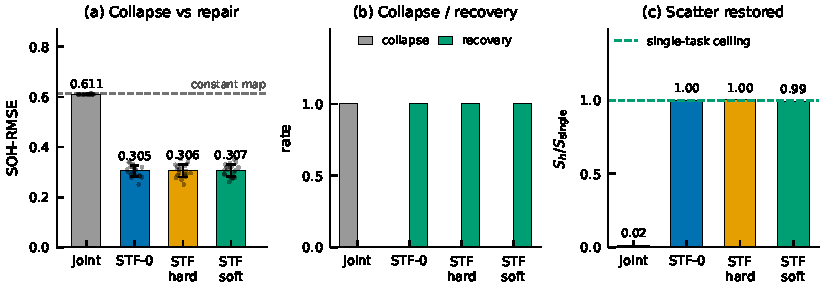
\includegraphics[width=\columnwidth]{figures/battery_repair.pdf}
\caption{Battery repair under the controlled unified protocol (NASA PCoE, $m=128$, $\alpha=10^4$, 20 seeds per mode). (a) Log-SOH RMSE on a linear axis: the mean decreases from $0.611$ to approximately $0.305$. (b) Collapse and task-recovery rates. (c) Scatter relative to the same-seed single-task reference; the dotted line marks $1.0$ and shading marks the operational collapse region below $0.3$. Small points are individual seeds; large markers and whiskers show means and population s.d. These log-SOH errors are not directly comparable with percentage-point SOH errors from the separate battery application.}
\label{fig:battery_repair}
\end{figure}

\begin{table}[t]
\centering
\caption{Filter-then-combiner experiments at high auxiliary doses (five seeds, three domains). Unfiltered branches retain collapse rates of $1.0$ and relative scatter at most $0.15$. The hard filter, alone or followed by PCGrad/CAGrad, avoids the collapse criterion in every seed. Primary metrics change modestly after composition; the reverse order was not tested. Bold identifies the filter-only reference within each block.}
\label{tab:compose}
\small
\resizebox{\columnwidth}{!}{\begin{tabular}{llcccccc}
\toprule
& & \multicolumn{3}{c}{unfiltered (\textsc{joint})} & \multicolumn{3}{c}{filtered (\textsc{stf-hard})} \\
\cmidrule(lr){3-5}\cmidrule(lr){6-8}
& combiner & sum & PCGrad & CAGrad & sum & PCGrad & CAGrad \\
\midrule
\multirow{3}{*}{Battery} & log-SOH RMSE$\downarrow$ & $0.611$ & $0.592$ & $0.603$ & $\mathbf{0.294}$ & $0.283$ & $0.291$ \\
 & collapse rate & $1.0$ & $1.0$ & $1.0$ & $0.0$ & $0.0$ & $0.0$ \\
 & relative scatter & $0.02$ & $0.03$ & $0.03$ & $\mathbf{1.00}$ & $1.05$ & $1.18$ \\
\midrule
\multirow{3}{*}{HAR} & accuracy$\uparrow$ & $0.941$ & $0.667$ & $0.952$ & $0.943$ & $0.933$ & $0.940$ \\
 & collapse rate & $1.0$ & $1.0$ & $1.0$ & $0.0$ & $0.0$ & $0.0$ \\
 & relative scatter & $0.15$ & $0.00$ & $0.03$ & $\mathbf{0.97}$ & $1.14$ & $1.03$ \\
\midrule
\multirow{3}{*}{RadioML} & accuracy$\uparrow$ & $0.293$ & $0.091$ & $0.109$ & $\mathbf{0.301}$ & $0.296$ & $0.295$ \\
 & collapse rate & $1.0$ & $1.0$ & $1.0$ & $0.0$ & $0.0$ & $0.0$ \\
 & relative scatter & $0.02$ & $0.00$ & $0.00$ & $\mathbf{0.97}$ & $0.99$ & $1.04$ \\
\bottomrule
\end{tabular}}
\end{table}

\begin{table}[t]
\centering
\caption{Anti-collapse regularizers at the doses and seeds of Table~\ref{tab:conflict} (ten seeds per configuration). Penalties of weight $\lambda$ are added to joint training. Entries report collapse rate, primary metric in parentheses, and relative scatter ($1.0$ is the single-task reference). Joint training, detachment, and hard filtering are evaluated in the same runs. Avoiding the scatter threshold need not improve the primary task.}
\label{tab:reg}
\small
\resizebox{\columnwidth}{!}{\begin{tabular}{lcccccc}
\toprule
 & \multicolumn{2}{c}{HAR} & \multicolumn{2}{c}{Battery} & \multicolumn{2}{c}{RadioML} \\
\cmidrule(lr){2-3}\cmidrule(lr){4-5}\cmidrule(lr){6-7}
 & coll.\ / acc.$\uparrow$ & rel.\ scat. & coll.\ / RMSE$\downarrow$ & rel.\ scat. & coll.\ / acc.$\uparrow$ & rel.\ scat. \\
\midrule
\textsc{joint} & $1.00$ ($0.945$) & $0.15$ & $1.00$ ($0.610$) & $0.022$ & $1.00$ ($0.256$) & $0.008$ \\
\textsc{stf-0} & $0.00$ ($0.945$) & $1.00$ & $0.00$ ($0.297$) & $1.00$ & $0.00$ ($0.341$) & $1.00$ \\
\textsc{stf-hard} & $0.00$ ($0.946$) & $0.99$ & $0.00$ ($0.299$) & $1.00$ & $0.00$ ($0.339$) & $0.97$ \\
\midrule
\multicolumn{7}{l}{\textit{VICReg (variance $+$ covariance)}} \\
\quad $\lambda{=}1$ & $1.00$ ($0.950$) & $0.22$ & $1.00$ ($0.610$) & $0.023$ & $1.00$ ($0.249$) & $0.007$ \\
\quad $\lambda{=}3$ & $0.20$ ($0.946$) & $0.31$ & $1.00$ ($0.610$) & $0.023$ & $1.00$ ($0.253$) & $0.007$ \\
\quad $\lambda{=}10$ & $0.00$ ($0.944$) & $0.36$ & $1.00$ ($0.609$) & $0.024$ & $1.00$ ($0.256$) & $0.008$ \\
\quad $\lambda{=}30$ & $0.00$ ($0.926$) & $0.36$ & $1.00$ ($0.604$) & $0.033$ & $1.00$ ($0.260$) & $0.008$ \\
\quad $\lambda{=}100$ & $0.00$ ($0.902$) & $0.36$ & $1.00$ ($0.451$) & $0.14$ & $1.00$ ($0.301$) & $0.011$ \\
\quad $\lambda{=}300$ & $0.00$ ($0.873$) & $0.36$ & $0.00$ ($0.339$) & $0.59$ & $1.00$ ($0.362$) & $0.035$ \\
\quad $\lambda{=}10^3$ & $0.00$ ($0.843$) & $0.36$ & $0.00$ ($0.390$) & $1.95$ & $1.00$ ($0.320$) & $0.15$ \\
\quad $\lambda{=}3\times10^3$ & $0.00$ ($0.831$) & $0.36$ & $0.00$ ($0.423$) & $3.70$ & $0.10$ ($0.207$) & $0.45$ \\
\quad $\lambda{=}10^4$ & $0.00$ ($0.821$) & $0.36$ & $0.00$ ($0.423$) & $4.54$ & $0.00$ ($0.215$) & $1.29$ \\
\midrule
\multicolumn{7}{l}{\textit{Barlow Twins (redundancy reduction)}} \\
\quad $\lambda{=}1$ & $1.00$ ($0.935$) & $0.11$ & $1.00$ ($0.607$) & $0.11$ & $1.00$ ($0.367$) & $0.016$ \\
\quad $\lambda{=}3$ & $1.00$ ($0.765$) & $0.022$ & $1.00$ ($0.607$) & $0.13$ & $1.00$ ($0.330$) & $0.024$ \\
\quad $\lambda{=}10$ & $1.00$ ($0.435$) & $0.006$ & $1.00$ ($0.606$) & $0.15$ & $1.00$ ($0.121$) & $0.074$ \\
\quad $\lambda{=}30$ & $1.00$ ($0.352$) & $0.006$ & $1.00$ ($0.606$) & $0.16$ & $1.00$ ($0.105$) & $0.096$ \\
\quad $\lambda{=}100$ & $1.00$ ($0.338$) & $0.006$ & $1.00$ ($0.605$) & $0.16$ & $1.00$ ($0.126$) & $0.072$ \\
\quad $\lambda{=}300$ & $1.00$ ($0.347$) & $0.006$ & $1.00$ ($0.606$) & $0.16$ & $1.00$ ($0.141$) & $0.043$ \\
\quad $\lambda{=}10^3$ & $1.00$ ($0.343$) & $0.006$ & $1.00$ ($0.606$) & $0.16$ & $1.00$ ($0.140$) & $0.042$ \\
\quad $\lambda{=}3\times10^3$ & $1.00$ ($0.365$) & $0.006$ & $1.00$ ($0.607$) & $0.16$ & $1.00$ ($0.148$) & $0.053$ \\
\quad $\lambda{=}10^4$ & $1.00$ ($0.339$) & $0.006$ & $1.00$ ($0.607$) & $0.16$ & $1.00$ ($0.153$) & $0.044$ \\
\bottomrule
\end{tabular}}
\end{table}

\subsection{Composition and Regime Weighting}

The following measurements expand the composition and weighting results in Sections~\ref{sec:bmtl} and~\ref{sec:conflict_ablations}.

At the tested high doses, applying PCGrad or CAGrad to the unfiltered battery branch leaves collapse rate at $1.0$ and relative scatter at $0.029/0.030$ (Table~\ref{tab:compose}). Hard filtering alone reduces collapse to $0.0$, restores relative scatter to $1.00$, and improves log-SOH RMSE from $0.611$ to $0.294$. Adding PCGrad or CAGrad afterward gives RMSE $0.283/0.291$ and scatter up to $1.18$. HAR and RadioML show the same qualitative preservation of scatter under composition. These results establish compatibility for the tested order; they neither show that sequencing is necessary nor establish why the unfiltered combiners fail.

BatteryMTL's multiplicative regime weights use training-data percentiles for C-rate and temperature, together with degradation rate. The aggregate SOH results change little, while factor ablations associate improvements in fast-charge and extreme-temperature windows with the rate and temperature terms, respectively (errors $0.95$ and $2.35$ when the corresponding terms are removed). Table~\ref{tab:bmtl} reports the historical aggregate results.

\subsection{Probe Dynamics During Training}\label{app:online}

The frozen calibration in Section~\ref{sec:stfcal} is motivated by the behavior of a continuously recomputed probe. We repeat unfiltered joint training with \texttt{--rho-trace}, using five seeds per configuration over 1730 HAR steps and 350 battery steps. Monitoring does not alter the measured trajectories: all 28 shared \textsc{bscale} configurations match exactly in task metric, collapse rate, relative scatter, and $\hat\rho$ (maximum difference zero).

Three observations matter. First, HAR probe values rise sharply during training: from $0.017$ to $1.9\times10^5$ at $m=32$, $0.010$ to $1.0\times10^5$ at $m=64$, and $0.006$ to $3.5\times10^4$ at $m=256$. Second, similar terminal values occur when the toxifier is inactive ($\alpha=0$) and at the lowest positive dose ($10^{-4}$), so a large probe value alone does not establish auxiliary-induced contraction. At $m=32$, increasing the dose instead lowers the terminal probe, to $5.3\times10^2$ at $10^{-2}$ and $1.1\times10^2$ at $3\times10^{-2}$. Third, in ten HAR configurations whose final scatter remains between $0.50$ and $1.04$ of the reference, the gate $\alpha\hat\rho\ge1$ opens in every seed between steps 110 and 590. A gate using this running statistic would therefore activate on some runs that never meet the collapse criterion.

Battery behaves differently: probe values remain $O(1)$, ranging from $0.29$--$0.49$ initially to $0.3$--$2.9$ at the final step. Among 35 seeds whose scatter stays above the half-height level, the gate opens only once, at the last step. These domain-dependent trajectories motivate a specified calibration time; they do not establish that a fixed probe is universally preferable to every adaptive rule. The script \texttt{repro/scripts/rho\_trace\_analyze.py} reproduces both analyses.

\subsection{Sensitivity to Calibration Time}\label{app:warmup}

The default calibration measures $\hat\rho$ after four detached warm-up epochs and fixes the gate and rank. We vary only this measurement time, $W\in\{1,2,4,8,16,32\}$, using five widths $32$--$512$ and ten seeds for HAR and battery, and four widths and ten seeds for NYUv2. The $W=4$ configuration exactly reproduces all 100 shared HAR and battery probe values. NYUv2 gives $2.258/2.008/1.637/1.285$, matching the rounded values in Appendix~\ref{app:nyu}.

Probe values depend on the training state. Across the warm-up sweep, HAR at $m=32$ increases from $0.63$ to $6.9\times10^4$, and at $m=512$ from $51.9$ to $1.6\times10^4$. Battery remains $O(1)$: $0.96$ to $1.92$ at $m=32$ and $0.058$ to $0.67$ at $m=512$. NYUv2 at $m=32$ changes from $1.94$ to $4.19$, a factor of $2.2$. Accordingly, width slopes fitted to $1/\hat\rho$ vary from $-2.00$ to $+0.55$ for HAR, $+0.37$ to $+0.97$ for battery, and $+0.11$ to $+0.27$ for NYUv2. These are calibration-dependent probe slopes, not interchangeable estimates of capacity scaling. Differences in primary-gradient magnitude, which appears in the denominator, can contribute to this sensitivity.

Measurement time also changes gate activation. For HAR at $m=64$, the inverse-mean probe value is $1.34$ at $W=1$, $0.181$ at $W=2$, $9.07\times10^{-3}$ at $W=4$, and $1.7\times10^{-5}$ at $W=32$, compared with the measured transition interval $[0.001,0.01]$. In the sixty-epoch, ten-seed experiment at $\alpha=0.03$, gates remain closed for $W=1$ and $W=2$: both settings collapse in $10/10$ seeds, with accuracy $0.947$ and relative scatter $0.19/0.20$, close to joint training ($0.949$, $0.19$). For $W\ge4$, all gates open, no seed collapses, and scatter returns to $0.99$--$1.00$. At $\alpha=100$, all six warm-up settings activate the gate and avoid collapse.

A short warm-up therefore fails at the marginal dose in this experiment. Detached warm-up also changes the training trajectory, so closed-gate runs need not equal joint training from initialization. Checking whether $\alpha\hat\rho\ge1$ verifies activation at the chosen operating dose; it does not independently validate protection. The script \texttt{repro/scripts/warmup\_sensitivity.py} reproduces these results.

\section{Anti-Collapse Regularizers at Matched Doses}\label{app:reg}

Table~\ref{tab:reg} evaluates two regularizer families at the doses and seeds of Table~\ref{tab:conflict}: VICReg's variance hinge plus off-diagonal covariance penalty, and Barlow Twins' redundancy-reduction penalty. Each is applied to the shared representation with weight $\lambda$. VICReg's invariance term is omitted because this experiment has no augmented-view pair. All rows use the same joint-training baseline; these are adaptations of the regularizers to this setting, not evaluations of their complete original learning pipelines.

Regularization can clear the operational collapse threshold without restoring the single-task reference or improving the task. In the coarse grid, VICReg first avoids collapse in all seeds at $\lambda=10$ for HAR, $300$ for battery, and $10000$ for RadioML. Barlow Twins does not do so at any tested weight.

On HAR, VICReg scatter stays near $0.36$ from $\lambda=10$ to $10^4$, while accuracy falls from $0.944$ to $0.821$. At the lowest clearing weight, accuracy is close to joint training ($0.945$) and detachment. On battery, scatter increases through the reference level, but the best tested RMSE is $0.339$ at $\lambda=300$ (relative scatter $0.59$), compared with $0.297$ for detachment. Larger weights worsen RMSE to $0.390$ at $10^3$ and $0.423$ at $10^4$; detachment is better in nine of ten seeds. On RadioML, $\lambda=10000$ gives zero collapse and scatter $1.29$, but accuracy drops to $0.215$, below both collapsed joint training ($0.256$) and detachment ($0.341$). These cases separate the scatter criterion from predictive utility.

The Barlow Twins adaptation yields absolute scatter as low as $0.011$, $0.012$, and $0.013$ for HAR, battery, and RadioML, respectively, or factors of $172$, $6$, and $24$ below their references. It fails to clear the collapse threshold throughout the tested grid, with HAR accuracy reaching approximately $0.34$--$0.44$ and RadioML approximately $0.11$ in the low-accuracy configurations.

Additional ten-seed sweeps use $\lambda\in\{2,5,20,50,200,500\}$ on HAR and $\lambda\in\{200,500,700,1500,2000,5000\}$ on battery. The recorded battery transition is bracketed by $150$ and $200$, and the lowest measured battery RMSE remains $0.339$ at $\lambda=300$, above detachment. HAR scatter remains near $0.36$ above its crossing. RadioML was not refined: the sampled collapse rate is $1.0$ at $1000$, $0.10$ at $3000$, and $0.0$ at $10000$. The experiments therefore locate an operational transition over a finite grid rather than a precise critical weight.

The collapse criterion thresholds relative scatter, whereas the regularized solution depends on the data, model, penalty, and its weight. Nothing in these objectives forces the resulting scatter to match the single-task reference. The tested grid therefore supports reporting representation statistics and task error together, rather than treating either as a sufficient measure of recovery.

\end{document}
